\documentclass[10pt,t]{beamer}
\usepackage{graphicx}
\setbeamersize{text margin left=10pt,text margin right=10pt}
%get rid of junk
\usetheme{default}
\beamertemplatenavigationsymbolsempty

% add packages to use
\usepackage{tabularx}
\usepackage{tikz}
\usetikzlibrary{trees,matrix,shapes,arrows}
\usetikzlibrary{calc}
\usepackage{fancyvrb}
\usepackage{listings}

\pgfdeclarelayer{background}
\pgfdeclarelayer{foreground}
\pgfsetlayers{background,main,foreground}
\usepackage{pgf,pgfarrows,pgfnodes,pgfautomata,pgfheaps,pgfshade}
\usepackage{amsmath,amssymb,amsfonts,subfigure,pifont}
\usepackage{multirow}
\usepackage{booktabs}
\usepackage{colortbl}
\usepackage{keystroke}
\usepackage{etex}


% named colors
%\definecolor{foreground}{RGB}{0,0,0}
\definecolor{background}{RGB}{241,231,200}
\definecolor{title}{RGB}{107,174,214}
\definecolor{gray}{RGB}{75,75,75}
%\definecolor{subtitle}{RGB}{102,255,204}
%\definecolor{hilight}{RGB}{102,255,204}
%\definecolor{vhilight}{RGB}{255,111,207}
%\definecolor{lolight}{RGB}{155,155,155}
\definecolor{lubrown}{RGB}{102,55,0}
\definecolor{lucream}{RGB}{241,231,200}
\definecolor{lugreen}{RGB}{195,207,33}
\definecolor{luyellow}{RGB}{255,196,35}
\definecolor{brown}{HTML}{502D0F}
\definecolor{lupurple}{RGB}{125,129,190}
\definecolor{lulime}{RGB}{217,226,219}
\definecolor{lublue}{RGB}{0,164,228}
\definecolor{lubg}{RGB}{241,231,200} % background color is lucream
%\definecolor{lubg}{RGB}{255,255,255} % background color is white

% The following color are for listing environment 
\definecolor{dkgreen}{rgb}{0,0.6,0}
%\definecolor{gray}{rgb}{0.5,0.5,0.5}
\definecolor{mauve}{rgb}{0.58,0,0.82}


\lstset{%
language=bash,                % the language of the code
basicstyle=\tiny\ttfamily,           % the size of the fonts that are used for the code
showspaces=false,               % show spaces adding particular underscores
showstringspaces=false,         % underline spaces within strings
showtabs=false,                 % show tabs within strings adding particular underscores
%frame=single,                   % adds a frame around the code
%rulecolor=\color{black},        % if not set, the frame-color may be changed on line-breaks within not-black text (e.g. comments (green here))
tabsize=2,                      % sets default tabsize to 2 spaces
%captionpos=b,                   % sets the caption-position to bottom
breaklines=true,                % sets automatic line breaking
breakatwhitespace=false,        % sets if automatic breaks should only happen at whitespace
%title=\lstname,                   % show the filename of files included with \lstinputlisting;
% also try caption instead of title
keywordstyle=\color{blue},          % keyword style
commentstyle=\color{dkgreen},       % comment style
stringstyle=\color{mauve},         % string literal style
escapeinside={!}{!},            % if you want to add LaTeX within your code
morekeywords={*,\dots,elif},              % if you want to add more keywords to the set
deletekeywords={\dots},              % if you want to delete keywords from the given language
%morecomment=[l]{//}
}
\lstset{%
language=csh,                % the language of the code
basicstyle=\tiny\ttfamily,           % the size of the fonts that are used for the code
showspaces=false,               % show spaces adding particular underscores
showstringspaces=false,         % underline spaces within strings
showtabs=false,                 % show tabs within strings adding particular underscores
%frame=single,                   % adds a frame around the code
%rulecolor=\color{black},        % if not set, the frame-color may be changed on line-breaks within not-black text (e.g. comments (green here))
tabsize=2,                      % sets default tabsize to 2 spaces
captionpos=b,                   % sets the caption-position to bottom
breaklines=true,                % sets automatic line breaking
breakatwhitespace=false,        % sets if automatic breaks should only happen at whitespace
%title=\lstname,                   % show the filename of files included with \lstinputlisting;
% also try caption instead of title
keywordstyle=\color{blue},          % keyword style
commentstyle=\color{dkgreen},       % comment style
stringstyle=\color{mauve},         % string literal style
escapeinside={\%*}{*)},            % if you want to add LaTeX within your code
morekeywords={*,\dots,elif},              % if you want to add more keywords to the set
deletekeywords={\dots},              % if you want to delete keywords from the given language
%morecomment=[l]{//}
}

\lstdefinestyle{LINUX}
{
    backgroundcolor=\color{white},
    basicstyle=\tiny\ttfamily,
    keywordstyle=\color{blue},
    morekeywords={apacheco,Tutorials,BASH,scripts,day1,examples},
    literate={>}{{\textcolor{blue}{>}}}1
         {/}{{\textcolor{blue}{/}}}1
         {./}{{\textcolor{black}{./ }}}1
         {~}{{\textcolor{blue}{\textasciitilde}}}1,
}


\DeclareSymbolFont{extraup}{U}{zavm}{m}{n}
%\DeclareMathSymbol{\vardiamond}{\mathalpha}{extraup}{87}
\newcommand{\cmark}{\ding{51}}
\newcommand{\xmark}{\ding{55}}
\newcommand{\smark}{\ding{77}}
\newcommand*\vardiamond{\textcolor{lubrown}{%
  \ensuremath{\blacklozenge}}}
\newcommand*\mybigstar{\textcolor{lubrown!90!yellow}{%
  \ensuremath{\bigstar}}}
\newcommand*\up{\textcolor{green!80!black}{%
  \ensuremath{\blacktriangle}}}
\newcommand*\down{\textcolor{red}{%
  \ensuremath{\blacktriangledown}}}
\newcommand*\const{\textcolor{darkgray}%
  {\textbf{--}}}
\newcommand*\enter{\tikz[baseline=-0.5ex] \draw[<-] (0,0) -| (0.5,0.1);}

\newcommand{\Verblubrown}[1]{\Verb[formatcom=\color{lubrown},fontseries=b,commandchars=\\\{\}]|#1|}
\newcommand{\Verblue}[1]{\Verb[formatcom=\color{lublue},fontseries=b,commandchars=\\\{\}]!#1!}
\newcommand{\Verbblue}[2][b]{\Verb[formatcom=\color{lublue},fontshape=#1,commandchars=\\\{\}]|#2|}
\newcommand{\Verblubrownp}[1]{\Verb[formatcom=\color{lubrown},fontseries=b,commandchars=\\\{\}]!#1!}


% use those colors
\setbeamercolor{titlelike}{fg=white,bg=lubrown}
\setbeamercolor{subtitle}{fg=lucream}
\setbeamercolor{author}{fg=lucream}
\setbeamercolor{institute}{fg=gray}
\setbeamercolor{normal text}{fg=black,bg=white}
\setbeamercolor{item}{fg=lubrown} % color of bullets
\setbeamercolor{subitem}{fg=gray}
\setbeamercolor{itemize/enumerate subbody}{fg=gray}
\setbeamertemplate{itemize subitem}{{\textendash}}
\setbeamerfont{itemize/enumerate subbody}{size=\footnotesize}
\setbeamerfont{itemize/enumerate subitem}{size=\footnotesize}
\setbeamercolor{footline}{bg=lubrown}

\setbeamercolor*{palette primary}{fg=lubrown,bg=white}
\setbeamercolor*{palette secondary}{bg=brown,fg=white} % footer
\setbeamercolor*{palette tertiary}{fg=lubrown,bg=white} % footer

% progressbar
\definecolor{lusteelgray}{HTML}{91A1AA}
\definecolor{luwarmgray}{HTML}{7D6A55}% background color for the progress bar

\makeatletter
\def\progressbar@progressbar{} % the progress bar
\newcount\progressbar@tmpcounta% auxiliary counter
\newcount\progressbar@tmpcountb% auxiliary counter
\newdimen\progressbar@pbht %progressbar height
\newdimen\progressbar@pbwd %progressbar width
\newdimen\progressbar@tmpdim % auxiliary dimension
\progressbar@pbwd=0.729\linewidth
\progressbar@pbht=1.87ex
%\progressbar@pbht=1.725ex
% the progress bar
\def\progressbar@progressbar{%
    \progressbar@tmpcounta= \insertframenumber % max = ?
    \progressbar@tmpcountb=\inserttotalframenumber      
    \progressbar@tmpdim=.5\progressbar@pbwd
    \multiply\progressbar@tmpdim by \progressbar@tmpcounta
    \divide\progressbar@tmpdim by \progressbar@tmpcountb
    \progressbar@tmpdim=2\progressbar@tmpdim
  \begin{tikzpicture}[rounded corners=0pt,very thin]
    \shade[top color=lubg,bottom color=lubg,middle color=lubg]
       (0pt, 0pt) rectangle ++ (\progressbar@pbwd, \progressbar@pbht);
%      \shade[draw=lusteelgray,top color=lusteelgray!50,bottom color=lusteelgray!50,middle color=lusteelgray] %
      \shade[draw=brown,top color=brown,bottom color=brown,middle color=brown] %
        (0pt, 0pt) rectangle ++ (\progressbar@tmpdim, \progressbar@pbht);
%    \draw[color=lubg]%normal text.fg!50]
%      (0pt, 0pt) rectangle (\progressbar@pbwd, \progressbar@pbht)
%        node[pos=0.5,color=normal text.fg] {\textnormal{%
%        }%
%    };
  \end{tikzpicture}%
}

% page number
%\setbeamertemplate{footline}{%
%    \raisebox{5pt}{\makebox[\paperwidth]{\hfill\makebox[20pt]{\color{lubrown}
%          \scriptsize\insertframenumber}}}\hspace*{5pt}}
\defbeamertemplate*{footline}{my footline}
{
    \ifnum \insertpagenumber=1
      \leavevmode%
      \hbox{%
      \begin{beamercolorbox}[wd=\paperwidth,ht=4.25ex,dp=1ex,center]{}%
        % empty environment to raise height
      \end{beamercolorbox}}%
      \vskip0pt%
    \else
      \leavevmode%
      \hbox{%
      \begin{beamercolorbox}[wd=.3\paperwidth,ht=2.0ex,dp=1ex,left]{date in head/foot}%
        %\usebeamerfont{date in head/foot}\raisebox{-1.5ex}{\includegraphics[width=0.3\paperwidth]{./LehighUniversityOnelineLogo}}\hfill
        \usebeamerfont{date in head/foot}\raisebox{-0.85ex}{\includegraphics[width=0.3\paperwidth]{./lulogo}}\hfill
      \end{beamercolorbox}%
      \begin{beamercolorbox}[wd=.61\paperwidth,ht=2.8ex,dp=0ex,center]{white}\raisebox{-1.1ex}{\progressbar@progressbar}%{date in head/foot}%
      \end{beamercolorbox}
      %\begin{beamercolorbox}[wd=.09\paperwidth,ht=2.8ex,dp=1ex,right]{date in head/foot}%
      \begin{beamercolorbox}[wd=.09\paperwidth,ht=2.75ex,dp=1ex,right]{date in head/foot}%
        \usebeamerfont{date in head/foot} \insertframenumber{} / \inserttotalframenumber\hspace*{2ex}
      \end{beamercolorbox}
      }%
      \vskip0pt%
    \fi
}

\defbeamertemplate*{footline}{myfootline}
{
  \leavevmode%
  \hbox{%
    \begin{beamercolorbox}[wd=\paperwidth,ht=4.25ex,dp=1ex,center]{}%
      % empty environment to raise height
  \end{beamercolorbox}}%
  \vskip0pt%
}

\setbeamertemplate{footline}[my footline]
%\setbeamersize{text margin left=10pt,text margin right=10pt}
%\setbeamersize{sidebar width left=5pt}
%\setbeamertemplate{sidebar canvas left}{\color{brown}\rule{5pt}{\paperheight}}
%\setbeamersize{sidebar width right=5pt}
%\setbeamertemplate{sidebar canvas right}{\color{brown}\rule{5pt}{\paperheight}}


\DeclareOptionBeamer{shadow}[true]{\def\beamer@themerounded@shadow{#1}}
\ExecuteOptionsBeamer{shadow=false}
\ProcessOptionsBeamer

\mode<presentation>

\setbeamertemplate{blocks}[rounded][shadow=\beamer@themerounded@shadow]
%\setbeamertemplate{items}[ball]
\setbeamertemplate{sections/subsections in toc}[ball]
\setbeamertemplate{title page}[default][colsep=-4bp,rounded=true,shadow=\beamer@themerounded@shadow]
\setbeamertemplate{part page}[default][colsep=-4bp,rounded=true,shadow=\beamer@themerounded@shadow]

\setbeamercolor{block title}{use=structure,fg=white,bg=structure.fg!75!black}
\setbeamercolor{block title alerted}{use=alerted text,fg=white,bg=alerted text.fg!75!black}
\setbeamercolor{block title example}{use=example text,fg=white,bg=example text.fg!75!black}

\setbeamercolor{block body}{parent=normal text,use=block title,bg=block title.bg!10!bg}
\setbeamercolor{block body alerted}{parent=normal text,use=block title alerted,bg=block title alerted.bg!10!bg}
\setbeamercolor{block body example}{parent=normal text,use=block title example,bg=block title example.bg!10!bg}

\mode<all>

\defbeamertemplate*{title page}{customized}[1][]
{ 
%%  \begin{flushright}
%%    \usebeamercolor[fg]{titlegraphic}\inserttitlegraphic\par
%%    \bigskip\vspace{0.4\paperheight}
%%    \usebeamerfont{title}\usebeamercolor[fg]{title}\inserttitle\par
%%    \usebeamerfont{subtitle}\usebeamercolor[fg]{subtitle}\insertsubtitle\par
%%    \bigskip
%%    \usebeamerfont{author}\insertauthor\par
%%    \usebeamerfont{institute}\insertinstitute\par
%%    \usebeamerfont{date}\insertdate\par
%%  \end{flushright}
%  \vfill
%  \hbox{
    \begin{flushright}
      \begin{beamercolorbox}[wd=\paperwidth,sep=8pt,right,#1]{title}
        \ifx\inserttitlegraphic\@empty
        \else
%        \vskip0.25em
               {\usebeamercolor[fg]{titlegraphic}\inserttitlegraphic}\hspace*{0.5cm}
               \fi
      \end{beamercolorbox}
      \vspace*{0.25\paperheight}
      \begin{beamercolorbox}[wd=\paperwidth,sep=8pt,right,#1]{title}
        \usebeamerfont{title}\inserttitle\hspace*{1cm}
        \ifx\insertsubtitle\@empty
        \else
        \vskip0.1pt
               {\usebeamerfont{subtitle}\usebeamercolor[fg]{subtitle}\insertsubtitle\hspace*{1cm}}
               \fi
      \end{beamercolorbox}
      \vspace*{0.15\paperheight}
      \begin{beamercolorbox}[wd=\paperwidth,sep=8pt,right,#1]{author}
        \usebeamerfont{author}\insertauthor\hspace*{1cm}\par
        \usebeamerfont{institute}\insertinstitute\hspace*{1cm}\par
        \usebeamerfont{date}\insertdate\hspace*{1cm}
      \end{beamercolorbox}
%      \vspace*{0pt}
%      \begin{beamercolorbox}[wd=\paperwidth,sep=8pt,right,#1]{institute}
%        \usebeamerfont{institute}\insertinstitute\hspace*{1cm}
%      \end{beamercolorbox}
%      \vspace*{0pt}
%      \begin{beamercolorbox}[wd=\paperwidth,sep=8pt,right,#1]{date}
%        \usebeamerfont{date}\insertdate\hspace*{1cm}
%      \end{beamercolorbox}  
    \end{flushright}
%  }
  \vskip0pt
}

% title page template
\setbeamertemplate{background canvas}{%
    \ifnum\c@framenumber=1%
        \color{lubrown}\rule{\paperwidth}{\paperheight}
    \else%
        \color{lubg}\rule{\paperwidth}{\paperheight}
    \fi%
}

% section page template
\defbeamertemplate*{section page}{mysection}[1][]
{
  \begin{centering} 
    \usebeamercolor[fg]{section title} 
    \usebeamerfont{section title} 
    \insertsection
    \par 
  \end{centering}   
}

\title{Shell Scripting}
\subtitle{Basic Commands \& Environment}
\author{Alexander B. Pacheco}
\institute{\href{http://researchcomputing.lehigh.edu}{LTS Research Computing}}%\\[2pt] \href{http://www.lehigh.edu}{Lehigh University}}
\date{March 19 \& 26, 2015}%\today}

% Delete this, if you do not want the table of contents to pop up at
% the beginning of each subsection:
\AtBeginSection[]
{
  \begingroup
  \setbeamertemplate{background canvas}[vertical shading][bottom=lubrown,top=lubrown]
  \setbeamertemplate{footline}[myfootline] 
  \setbeamertemplate{section page}[mysection]
  \frame[c]{
    \sectionpage
  }
  \endgroup
}

\titlegraphic{\includegraphics[scale=0.5]{lu}}
\begin{document}

\begin{frame}
  \titlepage
\end{frame}

\footnotesize
\begin{frame}[allowframebreaks]{Outline Day}
  \tableofcontents[part=1,hideallsubsections]
  \framebreak
  \tableofcontents[part=2,hideallsubsections]
\end{frame}

\begin{frame}[c]{Tutorial Outline}
  \begin{exampleblock}{Day 1: Basic Shell Scripting}
    \begin{itemize}
      \item[] On the first day, we will cover simple topics such as creating and executing simple shell scripts, arithmetic operations, loops and conditionals, command line arguments and functions.
        \ref{day1}
    \end{itemize}
  \end{exampleblock}
  \begin{exampleblock}{Day 2: Advanced Shell Scripting}
    \begin{itemize}
      \item[] On the second day, we will cover advanced topics such as creating shell scripts for data analysis which make use of tools such as regular expressions, grep, sed and the awk programming language.
    \end{itemize}
  \end{exampleblock}
\end{frame}

\part[Day 1]{Basic Shell Scripting}
\section{Overview of Introduction to Linux}
\begin{frame}[label=day1]
  \frametitle{Introduction}
  \begin{exampleblock}{What is a SHELL}
    \begin{itemize}
      \item The command line interface is the primary interface to Linux/Unix operating systems.
      \item Shells are how command-line interfaces are implemented in Linux/Unix.
      \item Each shell has varying capabilities and features and the user should choose the shell that best suits their needs.
      \item The shell is simply an application running on top of the kernel and provides a powerful interface to the system.
    \end{itemize}
  \end{exampleblock}
\end{frame}

\subsection{Types of Shell} 
\begin{frame}
  \frametitle{Types of Shell}
  \begin{itemize}
    \item[\texttt{sh}]: Bourne Shell
      \begin{enumerate}
      \item[$\vardiamond$] Developed by Stephen Bourne at AT\&T Bell Labs
      \end{enumerate}
    \item[\texttt{csh}]: C Shell
      \begin{enumerate}
      \item[$\vardiamond$] Developed by Bill Joy at University of California, Berkeley
      \end{enumerate}
    \item[\texttt{ksh}]: Korn Shell
      \begin{enumerate}
      \item[$\vardiamond$] Developed by David Korn at AT\&T Bell Labs
      \item[$\vardiamond$] backward-compatible with the Bourne shell and includes many features of the C shell
      \end{enumerate}
    \item[\texttt{bash}]: Bourne Again Shell
      \begin{enumerate}
      \item[$\vardiamond$] Developed by Brian Fox for the GNU Project as a free software replacement for the Bourne shell (sh).
      \item[$\vardiamond$] Default Shell on Linux and Mac OSX
      \item[$\vardiamond$] The name is also descriptive of what it did, bashing together the features of sh, csh and ksh
      \end{enumerate}
    \item[\texttt{tcsh}]: TENEX C Shell
      \begin{enumerate}
      \item[$\vardiamond$] Developed by Ken Greer at Carnegie Mellon University 
      \item[$\vardiamond$] It is essentially the C shell with programmable command line completion, command-line editing, and a few other features.
      \end{enumerate}
  \end{itemize}
\end{frame}

\begin{frame}
  \frametitle{Shell Comparison}
  \begin{center}
    \begin{columns}
      \column{0.65\textwidth}
      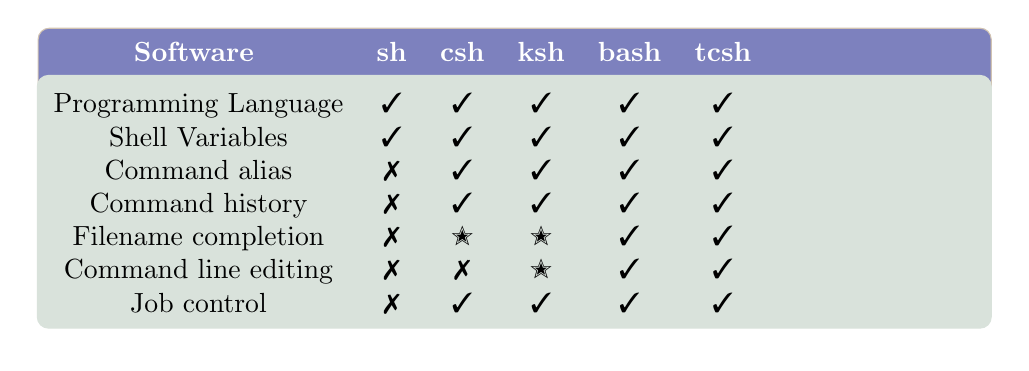
\begin{tikzpicture}
        \node (tbl) {
          \begin{tabularx}{\textwidth}{cccccc}
            \arrayrulecolor{tigersgold}
            \textcolor{white}{\textbf{Software} }& \textcolor{white}{\textbf{sh}} &\textcolor{white}{\textbf {csh}} & \textcolor{white}{\textbf{ksh}} & \textcolor{white}{\textbf{bash}} & \textcolor{white}{\textbf{tcsh}} \\
            Programming Language\rule{0pt}{3.5ex} & \cmark & \cmark & \cmark & \cmark & \cmark \\
            Shell Variables & \cmark & \cmark & \cmark & \cmark & \cmark \\
            Command alias & \xmark & \cmark & \cmark & \cmark & \cmark \\
            Command history & \xmark & \cmark & \cmark & \cmark & \cmark \\
            Filename completion & \xmark & \smark & \smark & \cmark & \cmark \\
            Command line editing & \xmark & \xmark & \smark & \cmark & \cmark \\
            Job control & \xmark & \cmark & \cmark & \cmark & \cmark \\
            [1.0ex]
        \end{tabularx}};
        \begin{pgfonlayer}{background}
          \draw[rounded corners,top color=lupurple,bottom color=lupurple,
            draw=lubrown!30] ($(tbl.north west)+(0.14,0)$)
          rectangle ($(tbl.north east)-(0.13,0.9)$);
          \draw[rounded corners,top color=lulime,bottom color=lulime,draw=lulime]
          ($(tbl.north east)-(0.13,0.6)$)
          rectangle ($(tbl.south west)+(0.13,0.2)$);
        \end{pgfonlayer}
      \end{tikzpicture}
      \begin{itemize}
      \item[\cmark]: Yes
      \item[\xmark]: No
      \item[\smark]: Yes, not set by default
      \item[] {\fontsize{6}{7}\selectfont\url{http://www.cis.rit.edu/class/simg211/unixintro/Shell.html}}
      \end{itemize}
    \end{columns}
  \end{center}
\end{frame}

\subsection{Variables}
\begin{frame}[fragile,allowframebreaks]
  \frametitle{Variables}
  \begin{itemize}
    \item A variable is a named object that contains data used by one or more applications. 
    \item There are two types of variables, Environment and User Defined and can contain  a number, character or a string of characters.
    \item Environment Variables provides a simple way to share configuration settings between multiple applications and processes in Linux.
%    \item By Convention, enviromental variables are often named using all uppercase letters
%    \item[e.g.] \texttt{PATH, LD\_LIBRARY\_PATH, LD\_INCLUDE\_PATH, TEXINPUTS, etc}
%    \item To reference a variable (environment or user defined) prepend \$ to the name of the variable
%    \item[e.g.] \texttt{\$PATH, \$LD\_LIBRARY\_PATH}
%    \item You can edit the environment variables.
%    \item Command to do this depends on the shell
%    \item[$\bigstar$] \texttt{To add your bin directory to the PATH variable}
%    \item[] \texttt{sh/ksh/bash}: \textbf{export PATH=\$\{HOME\}/bin:\$\{PATH\}}
%    \item[] \texttt{csh/tcsh}: \textbf{setenv PATH\,\,\$\{HOME\}/bin:\$\{PATH\}}
%    \item[$\bigstar$] \texttt{Note the syntax for the above commands}
%    \item[$\bigstar$] \textbf{sh/ksh/bash:} \texttt{no spaces except between export and PATH}
%    \item[$\bigstar$] \textbf{csh,tcsh:} \texttt{no = sign, just a space between PATH and the absolute path}
%    \item[$\bigstar$] \textbf{all shells:} \texttt{colon(:) to separate different paths and the variable that is appended to}
    \item As in programming languages like C, C++ and Fortran, defining your own variables makes the program or script extensible by you or a third party
    \item Rules for Variable Names
    \begin{enumerate}
%      \fontsize{7}{10}\selectfont{
        \item Variable names must start with a letter or underscore
        \item Number can be used anywhere else
        \item DO NOT USE special characters such as \texttt{@, \#, \%, \$}
        \item Case sensitive
        \item Examples
        \begin{itemize}
%          \fontsize{7}{10}\selectfont{
          \item Allowed: VARIABLE, VAR1234able, var\_name, \_VAR
          \item Not Allowed: 1VARIABLE, \%NAME, \$myvar, VAR@NAME 
%          }
        \end{itemize}
%      }
    \end{enumerate}
    \item To reference a variable, environment or user defined, you need to prepend the variable name with "\$" as in \$VARIABLE, \$PATH, etc.
    \item Its a good practice to protect your variable name within \{\dots\} such as \$\{PATH\} when referencing it. (We'll see an example in a few slides)
    \item Assigning value to a variable
    \begin{center}
      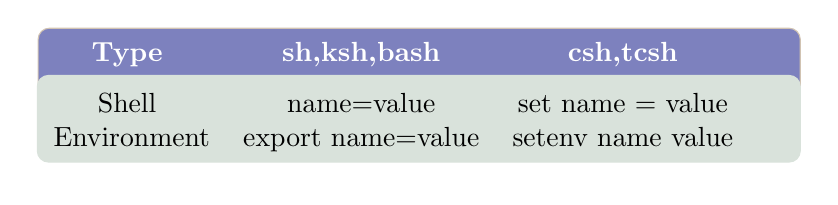
\begin{tikzpicture}
        \node (tbl) {
          \begin{tabularx}{0.8\textwidth}{ccc}
            \arrayrulecolor{tigersgold}
            \textcolor{white}{\textbf{Type} }& \textcolor{white}{\textbf{sh,ksh,bash}} &\textcolor{white}{\textbf {csh,tcsh}}\\
            Shell \rule{0pt}{3.5ex} & name=value & set name = value \\
            Environment & export name=value & setenv name value \\
            [1.0ex]
        \end{tabularx}};
        \begin{pgfonlayer}{background}
          \draw[rounded corners,top color=lupurple,bottom color=lupurple,
            draw=lubrown!30] ($(tbl.north west)+(0.14,0)$)
          rectangle ($(tbl.north east)-(0.13,0.9)$);
          \draw[rounded corners,top color=lulime,bottom color=lulime,draw=lulime]
          ($(tbl.north east)-(0.13,0.6)$)
          rectangle ($(tbl.south west)+(0.13,0.2)$);
        \end{pgfonlayer}
      \end{tikzpicture}
    \end{center}
    \item \textbf{sh,ksh,bash} THERE IS NO SPACE ON EITHER SIDE OF =
    \item \textbf{csh,tcsh} space on either side of = is allowed for the \texttt{set} command
    \item \textbf{csh,tcsh} There is no = in the \texttt{setenv} command
  \end{itemize}
\end{frame}

\subsection{File Permissions}
\begin{frame}[fragile, allowframebreaks]
  \frametitle{File Permissions}
  \begin{itemize}
    \item In *NIX OS's, you have three types of file permissions
    \begin{enumerate}
        \item read (r)
        \item write (w)
        \item execute (x)
    \end{enumerate}
    \item for three types of users
    \begin{enumerate}
        \item user
        \item group
        \item world i.e. everyone else who has access to the system
    \end{enumerate}
    \begin{exampleblock}{}
      \begin{tabular}{lllllllll}
        drwxr-xr-x. & 2 & user & user & 4096 & Jan & 28 & 08:27 & Public\\
        -rw-rw-r-\,-. & 1 & user & user & 3047 & Jan & 28 & 09:34 & README\\
      \end{tabular}
    \end{exampleblock}
    \item The first character signifies the type of the file
    \item[] \Verblubrown{d} for directory
    \item[] \Verblubrown{l} for symbolic link
    \item[] \Verblubrown{-} for normal file
    \item The next three characters of first triad signifies what the owner can do
    \item The second triad signifies what group member can do
    \item The third triad signifies what everyone else can do
      \begin{gather*}
        d\underbrace{rwx}_{u}\overbrace{r-x}^g\underbrace{r-x}_o
      \end{gather*}
    \item Read carries a weight of 4
    \item Write carries a weight of 2
    \item Execute carries a weight of 1
    \item The weights are added to give a value of 7 (rwx), 6(rw), 5(rx) or 3(wx) permissions. 
    \item \Verblubrown{chmod} is a *NIX command to change permissions on a file
    \item To give user rwx, group rx and world x permission, the command is
    \item[] \Verblubrown{chmod 751 filename}
    \item Instead of using numerical permissions you can also use symbolic mode
  \end{itemize}
  \begin{description}
    \item[u/g/o or a] user/group/world or all i.e. ugo
    \item[+/-] Add/remove permission
    \item[r/w/x] read/write/execute
  \end{description}
  \begin{itemize}
    \item Give everyone execute permission: 
    \item[] \Verblubrown{chmod a+x hello.sh }
    \item[] \Verblubrown{chmod ugo+x hello.sh}
    \item Remove group and world read \& write permission: 
    \item[] \Verblubrown{chmod go-rw hello.sh}
    \item Use the \Verblubrown{-R} flag to change permissions recursively, all files and directories and their contents.
    \item[] \Verblubrown{chmod -R 755 \$\{HOME\}/*}
    \item[] What is the permission on \$\{HOME\}?
  \end{itemize}
\end{frame}

\subsection{Input and Output}
\begin{frame}[fragile,allowframebreaks]
  \frametitle{Input/Output}
  \begin{itemize}
    \item The command \Verblubrown{echo} is used for displaying output to screen 
    \item For reading input from screen/keyboard/prompt
    \item[]\textbf{bash} \Verblubrown{read}
    \item[]\textbf{tcsh} \Verblubrown{\$<}
    \item The \Verblubrown{read} statement takes all characters typed until the \Enter \,key is pressed and stores them into a variable.
    \item[]Syntax \Verbblue{read <variable name>}
    \item[]Example \Verbblue{read name\Enter}
    \item[] \Verbblue{\textit{Alex Pacheco}}
    \item \Verblubrown{\$<} can accept only one argument. If you have multiple arguments, enclose the \Verblubrown{\$<} within quotes e.g. \Verblubrown{"\$<"}
    \item[]Syntax: \Verbblue{set <variable> = \$<}
    \item[]Example: \Verbblue{set name = "\$<"\Enter}
    \item[] \Verbblue{\textit{Alex Pacheco}}
    \item In the above examples, the name that you enter in stored in the variable \texttt{name}.
    \item Use the \Verblubrown{echo} command to print the variable \texttt{name} to the screen
    \item[] \Verbblue{echo \$name\Enter}
    \item The \Verblubrown{echo} statement can print multiple arguments. 
    \item By default, \Verblubrown{echo} eliminates redundant whitespace (multiple spaces and tabs) and replaces it with a single whitespace between arguments. 
    \item To include redundant whitespace, enclose the arguments within double quotes
    \item[] \texttt{echo Welcome to HPC\quad\quad Training}\enter\, (more than one space between HPC and Training)
    \item[] \texttt{echo "Welcome to HPC\quad\quad Training"}\enter
    \item[] \texttt{read name\enter} or \texttt{set name = "\$<"\enter}
    \item[] \textit{Alex\quad\quad\quad Pacheco\enter}
    \item[] \texttt{echo \$name\enter}
    \item[] \texttt{echo "\$name"\enter}
    \framebreak
    \item You can also use the \textbf{printf} command to display output
    \item[]Syntax: \texttt{printf <format> <arguments>}
    \item[]Example: \texttt{printf "\$name"\enter}
    \item[] \texttt{printf "\%s$\backslash$n" "\$name"\enter}
    \item Format Descriptors
    \begin{enumerate}
        \item[\%s] print argument as a string
        \item[\%d] print argument as an integer
        \item[\%f] print argument as a floating point number
        \item[$\backslash$n] print new line
        \item[] you can add a width for the argument between the \% and \{s,d,f\} fields
        \item[] \%4s, \%5d, \%7.4f
    \end{enumerate}
    \item The \textbf{printf} command is used in \textbf{awk} to print formatted data (more on this later) 
  \end{itemize}
\end{frame}

\begin{frame}
  \frametitle{I/O Redirection}
  \begin{itemize}
    \item There are three file descriptors for I/O streams
    \begin{enumerate}
        \item STDIN: Standard Input
        \item STDOUT: Standard Output
        \item STDERR: Standard Error
    \end{enumerate}
    \item 1 represents STDOUT and 2 represents STDOUT
    \item I/O redirection allows users to connect applications
    \begin{itemize}
      \item[$<$]: connects a file to STDIN of an application
      \item[$>$]: connects STDOUT of an application to a file
      \item[$> >$]: connects STDOUT of an application by appending to a file
      \item[$|$]: connects the STDOUT of an application to STDIN of another application.
    \end{itemize}
    \item Examples:
    \begin{enumerate}
      {\footnotesize
      \item write STDOUT to file: \texttt{ls -l > ls-l.out }
      \item write STDERR to file: \texttt{ls -l 2> ls-l.err }
      \item write STDOUT to STDERR: \texttt{ls -l 1>\&2 }
      \item write STDERR to STDOUT: \texttt{ls -l 2>\&1 }
      \item send STDOUT as STDIN: \texttt{ls -l | wc -l}
      }
    \end{enumerate}
  \end{itemize}
\end{frame}

%\begin{frame}{Exercise}
%  \begin{exampleblock}{}
%    \begin{itemize}
%      \item Create two shell variables containing
%      \begin{enumerate}
%        {\footnotesize
%          \item your name
%          \item[e.g.] MYNAME=Alex
%          \item a standard greeting
%          \item[e.g.] Greet=Hello
%          \item[] \texttt{echo \$MYNAME}\enter
%          \item[] \texttt{echo \$Greet}\enter
%          \item Combine and print your name and the greeting
%          \item[] \texttt{echo \$Greet \$MYNAME}\enter
%          \item What is the output of the following command?
%          \item[] \texttt{echo \$Greet \$MYNAME, Welcome to HPC Training}\enter
%        }
%      \end{enumerate}
%    \end{itemize}
%  \end{exampleblock}
%\end{frame}

\section{Shell Scripting Basics}
\subsection{Start Up Scripts}
\begin{frame}
  \frametitle{Start Up Scripts}
  \begin{itemize}
    \item When you login to a *NIX computer, shell scripts are automatically loaded depending on your default \texttt{shell}
    \item \textbf{sh,ksh}
    \begin{enumerate}
        \item \texttt{/etc/profile}
        \item \texttt{\$HOME/.profile}
    \end{enumerate}
    \item \textbf{bash}
    \begin{enumerate}
        \item \texttt{/etc/profile, login terminal only}
        \item \texttt{/etc/bashrc or /etc/bash/bashrc}
        \item \texttt{\$HOME/.bash\_profile, login terminal only}
        \item \texttt{\$HOME/.bashrc}
    \end{enumerate}
    \item \textbf{csh,tcsh}
    \begin{enumerate}
        \item \texttt{/etc/csh.cshrc}
        \item \texttt{\$HOME/.tcshrc}
        \item \texttt{\$HOME/.cshrc if .tcshrc is not present}
    \end{enumerate}
    \item The \texttt{.bashrc, .tcshrc, .cshrc, .bash\_profile} are script files where users can define their own aliases, environment variables, modify paths etc.
    \item e.g. the \texttt{alias rm="rm -i"} command will modify all \texttt{rm} commands that you type as \texttt{rm -i} 
  \end{itemize}
\end{frame}
\begin{frame}[fragile, allowframebreaks]
  \frametitle{Examples}
    \begin{block}{.bashrc}
      \begin{lstlisting}[language=bash]
# .bashrc

# Source global definitions
if [ -f /etc/bashrc ]; then
        . /etc/bashrc
fi

# User specific aliases and functions
alias c="clear"
alias rm="/bin/rm -i"
alias psu="ps -u apacheco"
alias em="emacs -nw"
alias ll="ls -lF"
alias la="ls -al"
export PATH=/home/apacheco/bin:${PATH}
export g09root=/home/apacheco/Software/Gaussian09
export GAUSS_SCRDIR=/home/apacheco/Software/scratch
source $g09root/g09/bsd/g09.profile

export TEXINPUTS=.:/usr/share/texmf//:/home/apacheco/LaTeX//:${TEXINPUTS}
export BIBINPUTS=.:/home/apacheco/TeX//:${BIBINPUTS}
      \end{lstlisting}
    \end{block}
    \begin{block}{.tcshrc}
      \begin{lstlisting}[language=csh]
# .tcshrc

# User specific aliases and functions
alias c clear
alias rm "/bin/rm -i"
alias psu "ps -u apacheco"
alias em "emacs -nw"
alias ll "ls -lF"
alias la "ls -al"
setenv PATH "/home/apacheco/bin:${PATH}"
setenv g09root "/home/apacheco/Software/Gaussian09"
setenv GAUSS_SCRDIR "/home/apacheco/Software/scratch"
source $g09root/g09/bsd/g09.login

setenv TEXINPUTS ".:/usr/share/texmf//:/home/apacheco/LaTeX//:${TEXINPUTS}"
setenv BIBINPUTS ".:/home/apacheco/TeX//:${BIBINPUTS}"
      \end{lstlisting}
    \end{block}
\end{frame}

\begin{frame}
  \frametitle{What is a scripting Language?}
  \begin{exampleblock}{}%{What is a Scripting Language?}
    \begin{itemize}
      \item A \textbf{scripting language} or \textbf{script language} is a \emph{programming language} that supports the writing of \textbf{scripts}.
      \item \textbf{Scripting Languages} provide a higher level of abstraction than standard programming languages.
      \item Compared to programming languages, scripting languages do not distinguish between data types: integers, real values, strings, etc.
      \item Scripting Languages tend to be good for automating the execution of other programs.
      \begin{enumerate}
          \item[$\vardiamond$] analyzing data
          \item[$\vardiamond$] running daily backups
      \end{enumerate}
      \item They are also good for writing a program that is going to be used only once and then discarded.
%    \end{itemize}
%  \end{exampleblock}
%  \begin{exampleblock}{What is a script?}
%    \begin{itemize}
      \item A \textbf{script} is a program written for a software environment that automate the execution of tasks which could alternatively be executed one-by-one by a human operator.
      \item The majority of script programs are ``quick and dirty'', where the main goal is to get the program written quickly.
    \end{itemize}
  \end{exampleblock}
\end{frame}

\subsection{Getting Started with Writing Simple Scripts}
\begin{frame}[fragile]
  \frametitle{Writing your first script}
  \vspace{-0.25cm}
  \begin{block}{Three things to do to write and execute a script}
    \begin{enumerate}
      \item Write a script
      \begin{itemize}
        \item A shell script is a file that contains ASCII text. 
        \item Create a file, \texttt{hello.sh} with the following lines 
      \end{itemize}
      \begin{lstlisting}[language=bash]
#!/bin/bash
# My First Script
echo "Hello World!"
      \end{lstlisting}
      \item Set permissions
      \begin{lstlisting}[style=LINUX]
~/Tutorials/BASH/scripts> chmod 755 hello.sh 
      \end{lstlisting}
      \item[] OR
      \begin{lstlisting}[style=LINUX]
~/Tutorials/BASH/scripts> chmod a+x hello.sh 
      \end{lstlisting}
      \item Execute the script
      \begin{lstlisting}[style=LINUX]
~/Tutorials/BASH/scripts> ./hello.sh 
Hello World!
      \end{lstlisting}
      \item If you do not set execute permission for the script, then
        \begin{lstlisting}[style=LINUX]
~/Tutorials/BASH/scripts> sh hello.sh
Hello World!
      \end{lstlisting}
    \end{enumerate}
  \end{block}
\end{frame}

\begin{frame}[fragile]
  \frametitle{Description of the script}
  \begin{itemize}
    \item My First Script
  \begin{lstlisting}[language=bash]
#!/bin/bash
# My First Script
echo "Hello World!"
  \end{lstlisting}
    \item The first line is called the "ShaBang'' line. It tells the OS which interpreter to use. In the current example, bash
    \item Other options are:
    \begin{enumerate}
        \item[$\vardiamond$] \texttt{sh\quad\,:   \#!/bin/sh}
        \item[$\vardiamond$] \texttt{ksh :  \#!/bin/ksh}
        \item[$\vardiamond$] \texttt{csh :  \#!/bin/csh}
        \item[$\vardiamond$] \texttt{tcsh: \#!/bin/tcsh}
    \end{enumerate}
    \item The second line is a comment. All comments begin with "\#".
    \item The third line tells the OS to print "Hello World!" to the screen.
  \end{itemize}
\end{frame}

\begin{frame}
  \frametitle{Special Characters}
  \begin{description}
    \item[\#:] starts a comment.
    \item[\$:] indicates the name of a variable.
    \item[$\backslash$:] escape character to display next character literally.
    \item[\{\quad\}:] used to enclose name of variable.
    \item[;] Command separator [semicolon]. Permits putting two or more commands on the same line.
    \item[;;] Terminator in a case option [double semicolon].
    \item[.] "dot" command [period]. Equivalent to source. This is a bash builtin.
    \item[\$?] exit status variable.
    \item[\$\$] process ID variable.
    \item[{[\quad]}] test expression
    \item[{[[\quad]]}] test expression, more flexible than [ ] 
    \item[{\$[\quad], ((\quad))}] integer expansion
    \item[$||$, \&\&, !] Logical OR, AND and NOT
  \end{description}

\end{frame}

\begin{frame}
  \frametitle{Quotation}
  \begin{itemize}
    \item Double Quotation \texttt{" "}
    \begin{itemize}
        \item Enclosed string is expanded ("\$", "/" and "`")
        \item Example: \texttt{echo "\$myvar"} prints the value of \texttt{myvar}
    \end{itemize}
    \item Single Quotation \texttt{' '}
    \begin{itemize}
        \item Enclosed string is read literally
        \item Example: \texttt{echo '\$myvar'} prints \texttt{\$myvar}
    \end{itemize}
    \item Back Quotation \texttt{` `}
    \begin{itemize}
        \item Used for command substitution
        \item Enclosed string is executed as a command
        \item Example: \texttt{echo `pwd`} prints the output of the \texttt{pwd} command i.e. print working directory
        \item In \textbf{bash}, you can also use \texttt{\$($\cdots$)} instead of \texttt{`$\cdots$`}
        \item[] e.g. \texttt{\$(pwd)} and \texttt{`pwd`} are the same
    \end{itemize}
  \end{itemize}
\end{frame}

\begin{frame}[fragile]{Example}
  \lstinputlisting[language=bash]{./scripts/day1/examples/quotes.sh}
  \begin{lstlisting}[basicstyle=\tiny\ttfamily,style=LINUX]
~/Tutorials/BASH/scripts/day1/examples> ./quotes.sh 
HI
Hello
$HI
Hello
$HI

HelloAlex
/home/apacheco/Tutorials/BASH/scripts/day1/examples
/home/apacheco/Tutorials/BASH/scripts/day1/examples
~/Tutorials/BASH/scripts/day1/examples>
  \end{lstlisting}
\end{frame}

\section{Beyond Basic Shell Scripting}
\subsection{Arithmetic Operations}
\begin{frame}[fragile,allowframebreaks]
  \frametitle{Arithmetic Operations}
  \begin{itemize}
    \item You can carry out numeric operations on integer variables
%  \end{itemize}
  \begin{columns}
    \column{0.5\textwidth}
    \begin{center}
      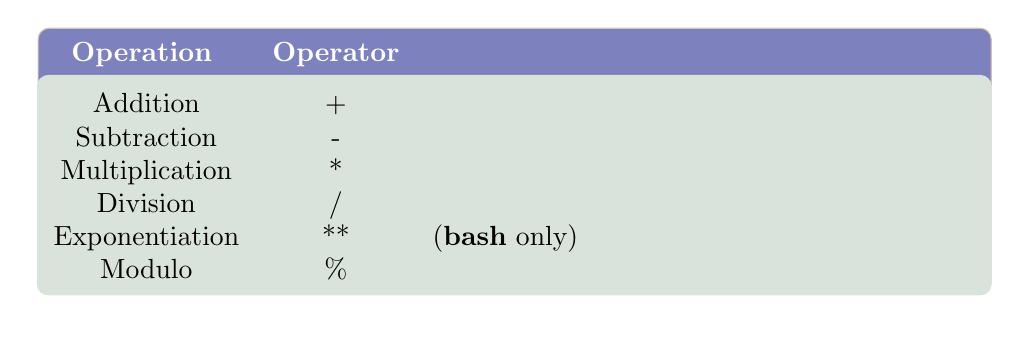
\begin{tikzpicture}
        \node (tbl) {
          \begin{tabularx}{\textwidth}{ccl}
            \arrayrulecolor{tigersgold}
            \textcolor{white}{\textbf{Operation} }& \textcolor{white}{\textbf{Operator}} & \\
            Addition\rule{0pt}{3.5ex} & + & \\
            Subtraction & - & \\
            Multiplication & * & \\
            Division & / \\
            Exponentiation & ** & (\textbf{bash} only)\\
            Modulo & \% & \\ 
            [1.0ex]
        \end{tabularx}};
        \begin{pgfonlayer}{background}
          \draw[rounded corners,top color=lupurple,bottom color=lupurple,
            draw=lubrown!30] ($(tbl.north west)+(0.14,0)$)
          rectangle ($(tbl.north east)-(0.13,0.9)$);
          \draw[rounded corners,top color=lulime,bottom color=lulime,draw=lulime]
          ($(tbl.north east)-(0.13,0.6)$)
          rectangle ($(tbl.south west)+(0.13,0.2)$);
        \end{pgfonlayer}
      \end{tikzpicture}
    \end{center}
  \end{columns}
%  \begin{itemize}
    \item Arithmetic operations in \textbf{bash} can be done within the \texttt{\$(($\cdots$))} or \texttt{\$[$\cdots$]} commands
    \begin{enumerate}
      \item[$\bigstar$] Add two numbers: \texttt{\$((1+2))}
      \item[$\bigstar$] Multiply two numbers: \texttt{\$[\$a*\$b]}
      \item[$\bigstar$] You can also use the \texttt{let} command: \texttt{let c=\$a-\$b}
      \item[$\bigstar$] or use the \texttt{expr} command: \texttt{c=`expr \$a - \$b`}
    \end{enumerate}
    \framebreak
    \item In \textbf{tcsh},
    \begin{enumerate}
      \item[$\bigstar$] Add two numbers: \texttt{@ x = 1 + 2}
      \item[$\bigstar$] Divide two numbers: \texttt{@ x = \$a / \$b}
      \item[$\bigstar$] You can also use the \texttt{expr} command: \texttt{set c = `expr \$a \% \$b`}
    \end{enumerate}
    \item Note the use of space
    \item[\textbf{bash}] space required around operator in the \texttt{expr} command
    \item[\textbf{tcsh}] space required between @ and variable, around = and numeric operators. 
    \item You can also use C-style increment operators
    \item[\textbf{bash}] \texttt{let c+=1} or \texttt{let c-{}-}
    \item[\textbf{tcsh}] \texttt{@ x -= 1} or \texttt{@ x++}
    \item[] \texttt{/=}, \texttt{*=} and \texttt{\%=} are also allowed.
    \item[\textbf{bash}]
    \item The above examples only work for integers.
    \item What about floating point number?
    \framebreak
    \item Using floating point in \textbf{bash} or \textbf{tcsh} scripts requires an external calculator like GNU \texttt{bc}.
    \begin{enumerate}
        \item[$\bigstar$] Add two numbers:
        \item[]\texttt{echo "3.8 + 4.2" | bc}
        \item[$\bigstar$] Divide two numbers and print result with a precision of 5 digits:
        \item[]\texttt{echo "scale=5; 2/5" | bc}
        \item[$\bigstar$] Call \texttt{bc} directly:
        \item[]\texttt{bc $<<<$ "scale=5; 2/5"}
        \item[$\bigstar$] Use \texttt{bc -l} to see result in floating point at max scale:
        \item[] \texttt{bc -l $<<<$ "2/5"}
    \end{enumerate}
    \item You can also use \textbf{awk} for floating point arithmetic. 
  \end{itemize}
\end{frame}


\subsection{Arrays}
\begin{frame}[fragile,allowframebreaks]
  \frametitle{Arrays}
  \begin{itemize}
    \item \textbf{bash} and \textbf{tcsh} supports one-dimensional arrays.
    \item Array elements may be initialized with the \texttt{variable[xx]} notation
    \item[] \texttt{variable[xx]=1}
    \item Initialize an array during declaration
    \item[\textbf{bash}] \texttt{name=(firstname 'last name')}
    \item[\textbf{tcsh}] \texttt{set name = (firstname 'last name')}
    \item reference an element \texttt{i} of an array \texttt{name}
    \item[] \texttt{\$\{name[i]\}}
    \item print the whole array
    \item[\textbf{bash}] \texttt{\$\{name[@]\}}
    \item[\textbf{tcsh}] \texttt{\$\{name\}}
    \item print length of array
    \item[\textbf{bash}] \texttt{\$\{\#name[@]\}}
    \item[\textbf{tcsh}] \texttt{\$\{\#name\}}
      \framebreak
    \item print length of element \texttt{i} of array \texttt{name}
    \item[] \texttt{\$\{\#name[i]\}}
    \item[] Note: In \textbf{bash} \texttt{\$\{\#name\}} prints the length of the first element of the array
    \item Add an element to an existing array
    \item[\textbf{bash}] \texttt{name=(title \$\{name[@]\})}
    \item[\textbf{tcsh}] \texttt{set name = ( title  "\$\{name\}")}
    \item In \textbf{tcsh} everything within "..." is one variable.
    \item In the above \textbf{tcsh} example, \texttt{title} is first element of new array while the second element is the old array \texttt{name}
    \item copy an array \texttt{name} to an array \texttt{user}
    \item[\textbf{bash}] \texttt{user=(\$\{name[@]\})}
    \item[\textbf{tcsh}] \texttt{set user = ( \$\{name\} )}
    \framebreak
    \item concatenate two arrays
    \item[\textbf{bash}] \texttt{nameuser=(\$\{name[@]\} \$\{user[@]\})}
    \item[\textbf{tcsh}] \texttt{set nameuser=( \$\{name\} \$\{user\} )}
    \item delete an entire array
    \item[] \texttt{unset name}
    \item remove an element \texttt{i} from an array
    \item[\textbf{bash}] \texttt{unset name[i]}
    \item[\textbf{tcsh}] \texttt{ @ j = \$i - 1}
    \item[ ] \texttt{ @ k =\$i + 1 }
    \item[ ] \texttt{ set name = ( \$\{name[1-\$j]\} \$\{name[\$k-]\})}
    \item[\textbf{bash}] the first array index is zero (0)
    \item[\textbf{tcsh}] the first array index is one (1)
  \end{itemize}
%  \framebreak
%  \begin{block}{Exercise}
%    \begin{enumerate}
%      \item Write a script to read your first and last name to an array.
%      \item Add your salutation and suffix to the array.
%      \item Drop either the salutation or suffix.
%      \item Print the array after each of the three steps above.
%    \end{enumerate}
%  \end{block}
  \framebreak
  \fontsize{5}{5.5}\selectfont{
    \begin{columns}
      \column{0.47\textwidth}
      \vspace{-0.5cm}
      \begin{exampleblock}{name.sh}
        \lstinputlisting[language=bash,basicstyle=\fontsize{3.5}{4.5}\selectfont\ttfamily]{./scripts/day1/examples/name.sh}
      \end{exampleblock}
    \column{0.47\textwidth}
      \vspace{-0.5cm}
      \begin{block}{name.csh}
        \lstinputlisting[language=csh,basicstyle=\fontsize{3.5}{4.5}\selectfont\ttfamily]{./scripts/day1/examples/name.csh}
      \end{block}
    \end{columns}
    \begin{columns}
      \column{0.47\textwidth}
%      \begin{exampleblock}{}
        \begin{lstlisting}[style=LINUX,basicstyle=\fontsize{3.5}{4.5}\selectfont\ttfamily]
~/Tutorials/BASH/scripts/day1/examples> ./name.sh 
Print your first and last name
Alex Pacheco
Hello  Alex Pacheco
Enter your salutation
Dr.
Enter your suffix
the first
Hello  Dr. Alex Pacheco the first
Hello  Dr. Alex the first
        \end{lstlisting}
%     \end{exampleblock}
      \column{0.47\textwidth}
%      \begin{block}{}
        \begin{lstlisting}[style=LINUX,basicstyle=\fontsize{3.5}{4.5}\selectfont\ttfamily]
~/Tutorials/BASH/scripts/day1/examples> ./name.csh 
Print your first name
Alex
Print your last name
Pacheco
Hello  Alex Pacheco
Enter your salutation
Dr.
Enter your suffix
the first
Hello  Dr. Alex Pacheco the first
Hello  Dr. Alex the first
        \end{lstlisting}
%      \end{block}
    \end{columns}
  }
\end{frame}

\subsection{Flow Control}
\begin{frame}
  \frametitle{Flow Control}
  \begin{itemize}
    \item Shell Scripting Languages execute commands in sequence similar to programming languages such as C, Fortran, etc.
    \item Control constructs can change the sequential order of commands.
    \item Control constructs available in \textbf{bash} and \textbf{tcsh} are
    \begin{enumerate}
%      {\scriptsize
        \item Conditionals: \texttt{if}
        \item Loops: \texttt{for, while, until}
        \item Switches: \texttt{case, switch}
%      }
    \end{enumerate}
  \end{itemize}
\end{frame}

\begin{frame}[fragile]
  \frametitle{\texttt{if} statement}
  \begin{itemize}
    \item An \texttt{if/then} construct tests whether the exit status of a list of commands is 0, and if so, executes one or more commands.
    \begin{columns}
      \column{5cm}
      \begin{exampleblock}{bash}
        \begin{lstlisting}[language=bash]
if [ condition1 ]; then
  some commands
elif [ condition2 ]; then
  some commands
else
  some commands
fi
        \end{lstlisting}
      \end{exampleblock}
      \column{5cm}
      \begin{block}{tcsh}
        \begin{lstlisting}[language=csh]
if ( condition1 ) then
  some commands
else if ( condition2 ) then
  some commands
else
  some commands
endif
        \end{lstlisting}
      \end{block}
    \end{columns}
  \item Note the space between \textit{condition} and "["\quad"]"
  \item \textbf{bash} is very strict about spaces.
  \item \textbf{tcsh} commands are not so strict about spaces.
  \item \textbf{tcsh} uses the \texttt{if-then-else if-else-endif} similar to Fortran.   
  \end{itemize}
\end{frame}

\begin{frame}
  \frametitle{Integer \& String Comparison Operators}
  \begin{exampleblock}{Integer Comparison}
    \begin{tabular}{lll}
      Operation & \textbf{bash} & \textbf{tcsh} \\
      \hline
      equal to & \texttt{if [ 1 -eq 2 ]} & \texttt{if (1 == 2)} \\
      not equal to & \texttt{if [ \$a -ne \$b ]} & \texttt{if (\$a != \$b)}\\
      greater than & \texttt{if [ \$a -gt \$b ]} & \texttt{if (\$a > \$b)}\\
      greater than or equal to & \texttt{if [ 1 -ge \$b ]} & \texttt{if (1 >= \$b)}\\
      less than & \texttt{if [ \$a -lt 2 ]} & \texttt{if (\$a < 2)}\\
      less than or equal to & \texttt{if [[ \$a -le \$b ]]} & \texttt{if (\$a <= \$b)} \\
      \hline
    \end{tabular}
  \end{exampleblock}
  \begin{exampleblock}{String Comparison}
    \begin{tabular}{lll}
      Operation & \textbf{bash} & \textbf{tcsh} \\
      \hline
      equal to & \texttt{if [ \$a == \$b ]} & \texttt{if (\$a == \$b)}\\
      not equal to & \texttt{if [ \$a != \$b ]} & \texttt{if (\$a != \$b)}\\
      zero length or null & \texttt{if [ -z \$a ] } & \texttt{if (\$\%a == 0)}\\
      non zero length & \texttt{if [ -n \$a ] } & \texttt{if (\$\%a > 0)}\\
      \hline
    \end{tabular}
  \end{exampleblock}
\end{frame}

\begin{frame}
  \frametitle{File Test \& Logical Operators}
  \begin{exampleblock}{File Test Operators}
    \begin{tabular}{lll}
      Operation & \textbf{bash} & \textbf{tcsh} \\
      \hline
      file exists & \texttt{if [ -e .bashrc ]} & \texttt{if ( -e .tcshrc )}\\
      file is a regular file & \texttt{if [ -f .bashrc ]} &  \\
      file is a directory & \texttt{if [ -d /home ]} & \texttt{if ( -d /home )} \\
      file is not zero size & \texttt{if [ -s .bashrc ]} & \texttt{if ( ! -z .tcshrc)} \\
      file has read permission & \texttt{ if [ -r .bashrc ]} & \texttt{ if ( -r .tcshrc)} \\
      file has write permission & \texttt{ if [ -w .bashrc ]} & \texttt{ if ( -w .tcshrc)} \\
      file has execute permission & \texttt{ if [ -x .bashrc ]} & \texttt{ if ( -x .tcshrc)} \\
      \hline
    \end{tabular}
  \end{exampleblock}
  \begin{exampleblock}{Logical Operators}
    \begin{tabular}{lll}
      Operation & \textbf{bash} & \textbf{tcsh} \\
      \hline
      NOT & \texttt{if [ ! -e .bashrc ]} & \texttt{if ( ! -z .tcshrc)} \\
      AND & \texttt{if [ \$a -eq 2 ] \&\& [ \$x -gt \$y ]} & \texttt{if (\$a == 2 \&\& \$x $<=$ \$y )} \\ 
      OR &  \texttt{if [[ \$a -eq 2 $||$  \$x -gt \$y ]]} & \texttt{if (\$a == 2 $||$ \$x $<=$ \$y )} \\
      \hline
    \end{tabular}
  \end{exampleblock}
\end{frame}

\begin{frame}[fragile]{Examples}
  \begin{itemize}
    \item Condition tests using the \texttt{if/then} may be nested
      \begin{columns}
        \column{0.5\textwidth}
        \begin{exampleblock}{}
      \begin{lstlisting}[language=bash]
read a
if [ "$a" -gt 0 ]; then
  if [ "$a" -lt 5 ]; then
    echo "The value of \"a\" lies somewhere between 0 and 5"
  fi
fi
      \end{lstlisting}
        \end{exampleblock}
        \column{0.45\textwidth}
        \begin{block}{}
      \begin{lstlisting}[language=csh]
set a = $<
if ( $a > 0 ) then
  if ( $a < 5 ) then
    echo "The value of $a lies somewhere between 0 and 5"
  endif
endif
      \end{lstlisting}
        \end{block}
      \end{columns}
    \item This is same as 
      \begin{columns}
        \column{0.5\textwidth}
        \begin{exampleblock}{}
      \begin{lstlisting}[language=bash]
read a
if [[ "$a" -gt 0 &&  "$a" -lt 5 ]]; then
  echo "The value of $a lies somewhere between 0 and 5"
fi
OR
if [ "$a" -gt 0 ] && [ "$a" -lt 5 ]; then
  echo "The value of $a lies somewhere between 0 and 5"
fi
      \end{lstlisting}
        \end{exampleblock}
        \column{0.45\textwidth}
        \begin{block}{}
      \begin{lstlisting}[language=csh]
set a = $<
if ( "$a" > 0  &&  "$a" < 5 ) then
  echo "The value of $a lies somewhere between 0 and 5"
endif
      \end{lstlisting}
        \end{block}
      \end{columns}
  \end{itemize}
\end{frame}

\begin{frame}
  \frametitle{Loop Constructs}
  \begin{itemize}
    \item A \textit{loop} is a block of code that iterates a list of commands as long as the \textit{loop control condition} is true.
    \item Loop constructs available in 
    \item[\textbf{bash}:] \texttt{for, while} and \texttt{until}
    \item[\textbf{tcsh}:] \texttt{foreach} and \texttt{while}
  \end{itemize}
\end{frame}

\begin{frame}[fragile]{bash: for loops}
  \begin{exampleblock}{}
    \begin{itemize}
      \item The \texttt{for} loop is the basic looping construct in \textbf{bash}
      \begin{lstlisting}[language=bash]
for arg in list
do
  some commands
done
      \end{lstlisting}
      \item the \texttt{for} and \texttt{do} lines can be written on the same line: \texttt{for} \textit{arg} in \textit{list}; \texttt{do}
      \item \texttt{for} loops can also use C style syntax
      \begin{lstlisting}[language=bash]
for (( EXP1; EXP2; EXP3 )); do
  some commands
done
      \end{lstlisting}
    \end{itemize}
  \end{exampleblock}
  \begin{columns}
    \column{0.3\textwidth}
    \begin{exampleblock}{}
      \begin{lstlisting}[language=bash]
for i in $(seq 1 10)
do
  touch file${i}.dat
done
      \end{lstlisting}
    \end{exampleblock}
    \column{0.35\textwidth}
    \begin{exampleblock}{}
      \begin{lstlisting}[language=bash]
for i in $(seq 1 10); do
  touch file${i}.dat
done
      \end{lstlisting}
    \end{exampleblock}
    \column{0.3\textwidth}
    \begin{exampleblock}{}
      \begin{lstlisting}[language=bash]
for ((i=1;i<=10;i++))
do
  touch file${i}.dat
done
      \end{lstlisting}
    \end{exampleblock}
  \end{columns}
\end{frame}

\begin{frame}[fragile]{tcsh: foreach loop}
  \begin{block}{}
    \begin{itemize}
      \item The \texttt{foreach} loop is the basic looping construct in \textbf{tcsh}
      \begin{lstlisting}
foreach arg (list)
  some commands
end
      \end{lstlisting}
    \end{itemize}
  \end{block}
  \begin{columns}
    \column{0.4\textwidth}
    \begin{block}{}
      \begin{lstlisting}
foreach i (`seq 1 10`)
  touch file$i.dat
end
      \end{lstlisting}
    \end{block}
  \end{columns}
\end{frame}

\begin{frame}[fragile]{while Construct}
  \begin{itemize}
%      \fontsize{7}{9}\selectfont{
  \item The \texttt{while} construct tests for a condition at the top of a loop, and keeps looping as long as that condition is true (returns a 0 exit status). 
  \item In contrast to a \texttt{for} loop, a \texttt{while} loop finds use in situations where the number of loop repetitions is not known beforehand.
  \end{itemize}
  \vspace{-0.5cm}
  \begin{columns}
    \column{0.4\textwidth}
    \begin{exampleblock}{bash}
      \begin{lstlisting}[language=bash]
while [ condition ]
do
  some commands
done
      \end{lstlisting}
    \end{exampleblock}
    \column{0.4\textwidth}
    \begin{block}{tcsh}
      \begin{lstlisting}[language=csh]
while ( condition )
  some commands
end
      \end{lstlisting}
    \end{block}
  \end{columns}
  \begin{columns}
    \column{0.4\textwidth}
    \vspace{-0.2cm}
    \begin{exampleblock}{factorial.sh}
      \lstinputlisting[language=bash]{./scripts/day1/examples/factorial.sh}
    \end{exampleblock}
    \column{0.4\textwidth}
    \vspace{-0.2cm}
    \begin{block}{factorial.csh}
      \lstinputlisting[language=csh]{./scripts/day1/examples/factorial.csh}
    \end{block}
  \end{columns}
\end{frame}

\begin{frame}[fragile]{until Contruct (bash only)}
  \begin{itemize}
  \item The \texttt{until} construct tests for a condition at the top of a loop, and keeps looping as long as that condition is false (opposite of \texttt{while} loop).
  \end{itemize}
  \begin{columns}
    \column{0.4\textwidth}
    \begin{exampleblock}{}
      \begin{lstlisting}[language=bash]
until [ condition is true ]
do
  some commands
done
      \end{lstlisting}
    \end{exampleblock}
  \end{columns}
  \begin{columns}
    \column{0.4\textwidth}
    \begin{exampleblock}{factorial2.sh}
      \lstinputlisting[language=bash]{./scripts/day1/examples/factorial2.sh}
    \end{exampleblock}
  \end{columns}
\end{frame}

\begin{frame}[fragile]{Nested Loops}
  \begin{itemize}
    \item \texttt{for, while \& until} loops can nested. To exit from the loop use the \texttt{break} command
  \end{itemize}
  \fontsize{5}{5}\selectfont{
    \begin{columns}
      \column{0.45\textwidth}
      \vspace{-0.2cm}
      \begin{exampleblock}{nestedloops.sh}
        \lstinputlisting[basicstyle=\fontsize{3.5}{4.5}\selectfont\ttfamily,language=bash]{./scripts/day1/examples/nestedloops.sh}
      \end{exampleblock}
      \column{0.45\textwidth}
      \vspace{-0.2cm}
      \begin{block}{nestedloops.csh}
        \lstinputlisting[basicstyle=\fontsize{3.5}{4.5}\selectfont\ttfamily,language=csh]{./scripts/day1/examples/nestedloops.csh}
      \end{block}
    \end{columns}
    \framebreak
    \begin{columns}
      \column{0.45\textwidth}
      \vspace{-0.2cm}
      \begin{exampleblock}{}
        \begin{lstlisting}[basicstyle=\fontsize{4}{5}\selectfont\ttfamily]
~/Tutorials/BASH/scripts/day1/examples> ./nestedloops.sh 
Nested for loops
Value of a in outer loop: 1
a * b = 1 * 1 = 1
a * b = 1 * 3 = 3
a * b = 1 * 5 = 5
Value of a in outer loop: 2
a * b = 2 * 1 = 2
a * b = 2 * 3 = 6
2 * 5 > 10
Value of a in outer loop: 3
a * b = 3 * 1 = 3
a * b = 3 * 3 = 9
3 * 5 > 10
Value of a in outer loop: 4
a * b = 4 * 1 = 4
4 * 3 > 10
Value of a in outer loop: 5
a * b = 5 * 1 = 5
5 * 3 > 10
========================

Nested for and while loops
Value of a in outer loop: 1
a * b = 1 * 1 = 1
a * b = 1 * 3 = 3
1 * 5 > 5
Value of a in outer loop: 2
a * b = 2 * 1 = 2
2 * 3 > 5
Value of a in outer loop: 3
a * b = 3 * 1 = 3
3 * 3 > 5
Value of a in outer loop: 4
a * b = 4 * 1 = 4
4 * 3 > 5
Value of a in outer loop: 5
5 * 1 > 5
========================
        \end{lstlisting}
      \end{exampleblock}
      \column{0.45\textwidth}
      \vspace{-0.2cm}
      \begin{block}{}
        \begin{lstlisting}[basicstyle=\fontsize{4}{5}\selectfont\ttfamily]
~/Tutorials/BASH/scripts> ./day1/examples/nestedloops.csh 
Nested for loops
Value of a in outer loop: 1
a * b = 1 * 1 = 1
a * b = 1 * 3 = 3
a * b = 1 * 5 = 5
Value of a in outer loop: 2
a * b = 2 * 1 = 2
a * b = 2 * 3 = 6
2 * 5 > 10
Value of a in outer loop: 3
a * b = 3 * 1 = 3
a * b = 3 * 3 = 9
3 * 5 > 10
Value of a in outer loop: 4
a * b = 4 * 1 = 4
4 * 3 > 10
Value of a in outer loop: 5
a * b = 5 * 1 = 5
5 * 3 > 10
========================

Nested for and while loops
Value of a in outer loop: 1
a * b = 1 * 1 = 1
a * b = 1 * 3 = 3
1 * 5 > 5
Value of a in outer loop: 2
a * b = 2 * 1 = 2
2 * 3 > 5
Value of a in outer loop: 3
a * b = 3 * 1 = 3
3 * 3 > 5
Value of a in outer loop: 4
a * b = 4 * 1 = 4
4 * 3 > 5
Value of a in outer loop: 5
5 * 1 > 5
========================
        \end{lstlisting}
      \end{block}
    \end{columns}
  }
\end{frame}

\begin{frame}[fragile,allowframebreaks]
  \frametitle{Switching or Branching Constructs}
  \begin{itemize}
    \fontsize{7}{9}\selectfont{
    \item The \texttt{case} and \texttt{select} constructs are technically not loops, since they do not iterate the execution of a code block. 
    \item Like loops, however, they direct program flow according to conditions at the top or bottom of the block.
    \begin{columns}
      \column{5cm}
      \begin{exampleblock}{\texttt{case} construct}
        \begin{lstlisting}[language=bash]
case variable in
  "condition1")
    some command
    ;;
  "condition2")
    some other command
    ;;
esac          
        \end{lstlisting}
      \end{exampleblock}
      \column{5cm}
      \begin{exampleblock}{\texttt{select} construct}
        \begin{lstlisting}[language=csh]
select variable [ list ]
do
  command
  break
done
        \end{lstlisting}
      \end{exampleblock}
    \end{columns}
    \framebreak
    \item \texttt{tcsh} has the \texttt{switch} construct
    \begin{columns}
      \column{5cm}
      \begin{exampleblock}{\texttt{switch} construct}
        \begin{lstlisting}[language=csh]
switch (arg list)
  case "variable"
    some command
    breaksw
endsw
        \end{lstlisting}
      \end{exampleblock}
    \end{columns}
    }
  \end{itemize}
\end{frame}

\begin{frame}[fragile]
  \begin{columns}
    \column{0.5\textwidth}
    \vspace{-0.5cm}
    \begin{exampleblock}{dooper.sh}
      \lstinputlisting[basicstyle=\fontsize{4}{4.5}\selectfont\ttfamily,language=bash]{./scripts/day1/examples/dooper.sh}
    \end{exampleblock}
    \column{0.4\textwidth}
    \vspace{-0.5cm}
    \begin{block}{dooper.csh}
      \lstinputlisting[basicstyle=\fontsize{4}{4.5}\selectfont\ttfamily,language=csh]{./scripts/day1/examples/dooper.csh}
    \end{block}
  \end{columns}
\end{frame}

\begin{frame}[fragile]
  \begin{columns}
    \column{0.48\textwidth}
%    \begin{exampleblock}{}
      \begin{lstlisting}[style=LINUX,basicstyle=\tiny\ttfamily]
~/Tutorials/BASH/scripts> ./day1/examples/dooper.sh
Print two numbers
1 4
What operation do you want to do?
1) add 3) multiply  5) exponentiate  7) all
2) subtract 4) divide  6) modulo   8) quit
#? 7
1 + 4 = 5
1 - 4 = -3
1 * 4 = 4
1 ** 4 = 1
1 / 4 = 0
1 % 4 = 1
#? 8
      \end{lstlisting}
%    \end{exampleblock}
    \column{0.48\textwidth}
%    \begin{block}{}
      \begin{lstlisting}[style=LINUX,basicstyle=\tiny\ttfamily]
~/Tutorials/BASH/scripts> ./day1/examples/dooper.csh 
Print two numbers one at a time
1
5
What operation do you want to do?
Enter +, -, x, /, % or all
all
1 + 5 = 6
1 - 5 = -4
1 * 5 = 5
1 / 5 = 0
1 % 5 = 1
        \end{lstlisting}
%    \end{block}
  \end{columns}
\end{frame}

\begin{frame}[fragile]
  \begin{columns}
    \column{0.48\textwidth}
    \begin{exampleblock}{dooper1.sh}
      \lstinputlisting[basicstyle=\fontsize{4}{4.5}\selectfont\ttfamily,language=bash]{./scripts/day1/examples/dooper1.sh}
    \end{exampleblock}
    \column{0.48\textwidth}
    \begin{lstlisting}[style=LINUX,basicstyle=\tiny\ttfamily]
~/Tutorials/BASH/scripts> ./day1/examples/dooper1.sh
Print two numbers
2 5
What operation do you want to do?
Options are add, subtract, multiply, exponentiate, divide, modulo and all
all
2 + 5 = 7
2 - 5 = -3
2 * 5 = 10
2 ** 5 = 32
2 / 5 = 0
2 % 5 = 2
    \end{lstlisting}
  \end{columns}
\end{frame}


\subsection{Command Line Arguments}
\begin{frame}
  \frametitle{Command Line Arguments}
  \begin{itemize}
    \item Similar to programming languages, \texttt{bash} (and other shell scripting languages) can also take command line arguments
    \begin{itemize}
      \item \texttt{./scriptname arg1 arg2 arg3 arg4 ...}
      \item \texttt{\$0,\$1,\$2,\$3, etc}: positional parameters corresponding to \texttt{./scriptname,arg1,arg2,arg3,arg4,...} respectively  
      \item \texttt{\$\#}: number of command line arguments
      \item \texttt{\$*}: all of the positional parameters, seen as a single word
      \item \texttt{\$@}: same as \texttt{\$*} but each parameter is a quoted string.
      \item \texttt{shift N}: shift positional parameters from \texttt{N+1} to \texttt{\$\#} are renamed to variable names from \texttt{\$1} to \texttt{\$\# - N + 1}
    \end{itemize}
    \item In \texttt{csh,tcsh}
    \begin{itemize}
      \item an array \texttt{argv} contains the list of arguments with \texttt{argv[0]} set to name of script.
      \item \texttt{\#argv} is the number of arguments i.e. length of \texttt{argv} array.
    \end{itemize}
  \end{itemize}
\end{frame}

\begin{frame}[fragile]
  \begin{columns}
    \column{0.48\textwidth}
    \vspace{-0.5cm}
    \begin{exampleblock}{shift.sh}
      \lstinputlisting[language=bash,basicstyle=\fontsize{3.5}{4.5}\selectfont\ttfamily]{./scripts/day1/examples/shift.sh}
    \end{exampleblock}
    \column{0.48\textwidth}
    \vspace{-0.5cm}
    \begin{block}{shift.csh}
      \lstinputlisting[language=csh,basicstyle=\fontsize{3.5}{4.5}\selectfont\ttfamily]{./scripts/day1/examples/shift.csh}
    \end{block}
  \end{columns}
  \begin{columns}
    \column{0.48\textwidth}
%    \begin{exampleblock}{}
      \begin{lstlisting}[style=LINUX,basicstyle=\fontsize{3.5}{4.5}\selectfont\ttfamily]
dyn100085:examples apacheco$ ./shift.sh $(seq 1 5)
Number of Arguments:  5
List of Arguments:  1 2 3 4 5
Name of script that you are running:  ./shift.sh
Command You Entered: ./shift.sh 1 2 3 4 5
Argument List is:  1 2 3 4 5
Number of Arguments:  5
Argument List is:  2 3 4 5
Number of Arguments:  4
Argument List is:  3 4 5
Number of Arguments:  3
Argument List is:  4 5
Number of Arguments:  2
Argument List is:  5
Number of Arguments:  1
      \end{lstlisting}
%    \end{exampleblock}
    \column{0.48\textwidth}
%    \begin{block}{}
      \begin{lstlisting}[style=LINUX,basicstyle=\fontsize{3.5}{4.5}\selectfont\ttfamily]
dyn100085:examples apacheco$ ./shift.csh $(seq 1 5)
Number of Arguments:  5
List of Arguments:  1 2 3 4 5
Name of script that you are running:  ./shift.csh
Command You Entered: ./shift.csh 1 2 3 4 5
Argument List is:  1 2 3 4 5
Number of Arguments:  5
Argument List is:  2 3 4 5
Number of Arguments:  4
Argument List is:  3 4 5
Number of Arguments:  3
Argument List is:  4 5
Number of Arguments:  2
Argument List is:  5
Number of Arguments:  1
      \end{lstlisting}
%    \end{block}
  \end{columns}
\end{frame}

\begin{frame}[fragile]{Declare command}
  \begin{itemize}
    \item Use the \textbf{declare} command to set variable and functions attributes.
    \item Create a constant variable i.e. read only variable
    \item[] \Verblubrown{Syntax:}
    \item[] \Verbblue{declare -r var}
    \item[] \Verbblue{declare -r varName=value}
    \item Create an integer variable
    \item[] \Verblubrown{Syntax:} 
    \item[] \Verbblue{declare -i var}
    \item[] \Verbblue{declare -i varName=value}
    \item You can carry out arithmetic operations on variables declared as integers
  \end{itemize}
  \begin{columns}
    \column{8cm}
%    \begin{exampleblock}{}
      \begin{lstlisting}[style=LINUX]
~/Tutorials/BASH> j=10/5 ; echo $j
10/5
~/Tutorials/BASH> declare -i j; j=10/5 ; echo $j
2
      \end{lstlisting}
%    \end{exampleblock}
  \end{columns}
\end{frame}
\subsection{Functions}
\begin{frame}[fragile,allowframebreaks]{Functions}
  \begin{itemize}
    \item Like "real" programming languages, \textbf{bash} has functions.
    \item A function is a subroutine, a code block that implements a set of operations, a "black box" that performs a specified task. 
    \item Wherever there is repetitive code, when a task repeats with only slight variations in procedure, then consider using a function.
  \end{itemize}
  \begin{columns}
    \column{5cm}
    {\scriptsize
      \begin{exampleblock}{}
        \begin{lstlisting}[language=bash]
function function_name {
  command
}
OR
function_name () {
  command
}
        \end{lstlisting}
      \end{exampleblock}
    }
  \end{columns}
  \framebreak
    \begin{columns}
      \column{0.45\textwidth}
      \begin{exampleblock}{shift10.sh}
        \lstinputlisting[language=bash,basicstyle=\fontsize{4}{4.5}\selectfont\ttfamily]{./scripts/day1/examples/shift10.sh}
      \end{exampleblock}
      \column{0.53\textwidth}
%      \begin{exampleblock}{}
        \begin{lstlisting}[style=LINUX,basicstyle=\fontsize{4}{4.5}\selectfont\ttfamily]
dyn100085:examples apacheco$ ./shift10.sh
USAGE: ./shift10.sh [atleast 11 arguments]
dyn100085:examples apacheco$ ./shift10.sh $(seq 1 10)
USAGE: ./shift10.sh [atleast 11 arguments]
dyn100085:examples apacheco$ ./shift10.sh `seq 1 2 22`
Number of Arguments:  11
List of Arguments:  1 3 5 7 9 11 13 15 17 19 21
Name of script that you are running:  ./shift10.sh
Command You Entered: ./shift10.sh 1 3 5 7 9 11 13 15 17 19 21
First Argument 1
Tenth and Eleventh argument 10 11 19 21
Argument List is:  1 3 5 7 9 11 13 15 17 19 21
Number of Arguments:  11
Argument List is:  19 21
Number of Arguments:  2
dyn100085:examples apacheco$ ./shift10.sh $(seq 21 2 44)
Number of Arguments:  12
List of Arguments:  21 23 25 27 29 31 33 35 37 39 41 43
Name of script that you are running:  ./shift10.sh
Command You Entered: ./shift10.sh 21 23 25 27 29 31 33 35 37 39 41 43
First Argument 21
Tenth and Eleventh argument 210 211 39 41
Argument List is:  21 23 25 27 29 31 33 35 37 39 41 43
Number of Arguments:  12
Argument List is:  39 41 43
Number of Arguments:  3
        \end{lstlisting}
%      \end{exampleblock}
    \end{columns}
  \framebreak
  \begin{itemize}
    \item You can also pass arguments to a function.
    \item All function parameters or arguments can be accessed via \$1, \$2, \$3,..., \$N.
    \item \$0 always point to the shell script name.
    \item \$* or \$@ holds all parameters or arguments passed to the function.
    \item \$\# holds the number of positional parameters passed to the function.
    \item Array variable called \texttt{FUNCNAME} contains the names of all shell functions currently in the execution call stack.
    \item By default all variables are global.
    \item Modifying a variable in a function changes it in the whole script.
    \item You can create a local variables using the \textbf{local} command
    \item[] \Verblubrown{Syntax:}
    \item[] \Verbblue{local var=value}
    \item[] \Verbblue{local varName}
  \end{itemize}
  \framebreak
  \begin{itemize}
    \item A function may recursively call itself even without use of local variables.
  \end{itemize}
  \fontsize{7}{9}\selectfont{
    \begin{columns}
      \column{0.45\textwidth}
      \vspace{-0.35cm}
      \begin{exampleblock}{factorial3.sh}
        \lstinputlisting[basicstyle=\fontsize{4}{4.5}\selectfont\ttfamily,language=bash]{./scripts/day1/examples/factorial3.sh}
      \end{exampleblock}
      \column{0.53\textwidth}
%      \vspace{-0.35cm}
%      \begin{exampleblock}{}
        \begin{lstlisting}[style=LINUX,basicstyle=\fontsize{4}{4.5}\selectfont\ttfamily]
dyn100085:examples apacheco$ ./factorial3.sh $(seq 1 2 11)
Factorial of 1 is 1
Factorial of 3 is 6
Factorial of 5 is 120
Factorial of 7 is 5040
Factorial of 9 is 362880
Factorial of 11 is 39916800
        \end{lstlisting}
%      \end{exampleblock}
    \end{columns}
  }
\end{frame}

%\section{Advanced Topics Preview}
%\begin{frame}
%  \frametitle{grep \& egrep}
%  \begin{itemize}
%    \item \texttt{grep} is a Unix utility that searches through either information piped to it or files in the current directory.
%    \item \texttt{egrep} is extended grep, same as \texttt{grep -E}
%    \item Use \texttt{zgrep} for compressed files.
%    \item Usage: \texttt{grep <options> <search pattern> <files>} 
%    \item Commonly used options
%    \begin{itemize}
%      {\scriptsize
%      \item[-i]: ignore case during search
%      \item[-r]: search recursively
%      \item[-v]: invert match i.e. match everything except pattern
%      \item[-l]: list files that match pattern
%      \item[-L]: list files that do not match pattern
%      \item[-n]: prefix each line of output with the line number within its input file.
%      }
%    \end{itemize}
%  \end{itemize}
%\end{frame}

%\begin{frame}
%  \frametitle{sed}
%  \begin{itemize}
%    \item sed ("stream editor") is Unix utility for parsing and transforming text files.
%    \item sed is line-oriented, it operates one line at a time and allows regular expression matching and substitution.
%    \item The most commonly used feature of sed is the 's' (substitution command)
%    \begin{enumerate}
%      \item[$\vardiamond$] echo Auburn Tigers | sed 's/Auburn/LSU/g'
%      \item[$\bigstar$] Add the \texttt{-e} to carry out multiple matches.
%      \item[$\vardiamond$] echo LSU Tigers | sed -e 's/LSU/LaTech/g' -e 's/Tigers/Bulldogs/g'
%      \item[$\bigstar$] insert a blank line above and below the lines that match regex: 
%      \item[]\texttt{sed '/regex/\{x;p;x;G;\}'}
%      \item[$\bigstar$] delete all blank lines in a file: \texttt{sed '/\^{}\$/d'}
%      \item[$\bigstar$] delete lines n through m in file: \texttt{sed 'n,md'}
%      \item[$\bigstar$] delete lines matching pattern regex: \texttt{sed '/regex/d'}
%      \item[$\bigstar$]print only lines which match regular expression: \texttt{sed -n '/regex/p'}
%      \item[$\bigstar$] print section of file between two regex: \texttt{sed -n '/regex1/,/regex2/p'}
%      \item[$\bigstar$] print section of file from regex to enf of file: \texttt{sed -n '/regex1/,\$p'}
%     \end{enumerate}
%    \item sed one-liners: \url{http://sed.sourceforge.net/sed1line.txt}
%   \end{itemize}
%\end{frame}

%\begin{frame}
%  \frametitle{awk}
%  \begin{itemize}
%    \item The Awk text-processing language is useful for such tasks as:
%    \begin{enumerate}
%      \item[$\bigstar$] Tallying information from text files and creating reports from the results.
%      \item[$\bigstar$]Adding additional functions to text editors like "vi".
%      \item[$\bigstar$] Translating files from one format to another.
%      \item[$\bigstar$] Creating small databases.
%      \item[$\bigstar$]Performing mathematical operations on files of numeric data.
%    \end{enumerate}
%    \item Awk has two faces: 
%    \begin{enumerate}
%      \item[$\bigstar$] it is a utility for performing simple text-processing tasks, and 
%      \item[$\bigstar$] it is a programming language for performing complex text-processing tasks.
%    \end{enumerate}
%    \item Simplest form of using awk
%    \begin{enumerate}
%      \item[$\vardiamond$]\textbf{awk} \textit{search pattern} \{\texttt{program actions}\}
%      \item[$\vardiamond$] Most command action: \texttt{print}
%      \item[$\vardiamond$] Print file dosum.sh: \texttt{awk '\{print \$0\}' dosum.sh}
%      \item[$\vardiamond$] Print line matching bash in all files in current directory:
%      \item[] \texttt{awk '/bash/\{print \$0\}' *.sh }
%    \end{enumerate}
%    \item \textbf{awk} supports the if conditional and for loops
%    \item[] \texttt{awk '\{ if (NR > 0)\{print "File not empty"\}\}' hello.sh}
%    \item[] \texttt{awk '\{for (i=1;i<=NF;i++)\{print \$i\}\}' name.sh}
%    \item[] \texttt{ls *.sh | awk -F. '\{print \$1\}'}
%    \item[] NR$\equiv$Number of records; NF$\equiv$Number of fields (or columns)
%    \item awk one-liners: \url{http://www.pement.org/awk/awk1line.txt}
%  \end{itemize}
%\end{frame}

\begin{frame}
  \frametitle{Scripting for Job Submission}
  \begin{block}{Problem Description}
    \begin{itemize}
      \item I have to run more than one serial job.
        \begin{itemize}
          \item Solution: Create a script that will submit and run multiple serial jobs.
        \end{itemize}
      \item I don't want to submit multiple jobs using the serial queue since
        \begin{itemize}
          \item Cluster Admins give lower priority to jobs that are not parallelized
          \item The number of jobs that I want to run exceed the maximum number of jobs that I can run simultaneously
        \end{itemize}
      \item How do I submit \emph{one} job which can run multiple serial jobs?
    \end{itemize}
  \end{block}
  \begin{exampleblock}{One Solution of many}
    \begin{itemize}
      \item Write a script which will log into all unique nodes and run your serial jobs in background.
      \item Easy said than done
      \item What do you need to know?
      \begin{enumerate}
        \fontsize{8}{7}\selectfont{
          \item Shell Scripting
          \item How to run a job in background
          \item Know what the \texttt{wait} command does
        }
      \end{enumerate}
    \end{itemize}
  \end{exampleblock}
\end{frame}

\begin{frame}[fragile]
  \begin{lstlisting}[language=bash]
[alp514@corona1 ~]$ cat checknodes.pbs 
#!/bin/bash
#
#PBS -q normal
#PBS -l nodes=4:ppn=16
#PBS -l walltime=00:30:00
#PBS -V
#PBS -o nodetest.out
#PBS -e nodetest.err
#PBS -N testing
#PBS -M alp514@lehigh.edu
#PBS -m abe
#

export WORK_DIR=$PBS_O_WORKDIR
export NPROCS=`wc -l $PBS_NODEFILE |gawk '//{print $1}'`

NODES=(`cat ``$PBS_NODEFILE''` )
UNODES=(`uniq ``$PBS_NODEFILE''` )

echo ``Nodes Available: `` ${NODES[@]}
echo ``Unique Nodes Available: `` ${UNODES[@]}

echo ``Get Hostnames for all processes''
i=0
for nodes in ``${NODES[@]}''; do
  ssh -n $nodes 'echo $HOSTNAME '$i' ' &
  let i=i+1
done
wait

echo ``Get Hostnames for all unique nodes''
i=0
NPROCS=`uniq $PBS_NODEFILE | wc -l |gawk '//{print $1}'`
let NPROCS-=1
while [ $i -le $NPROCS ] ; do
  ssh -n ${UNODES[$i]} 'echo $HOSTNAME '$i' '
  let i=i+1
done

[alp514@corona1 ~]$ qsub checknodes.pbs
688825.corona1.cc.lehigh.edu
  \end{lstlisting}
\end{frame}

\begin{frame}[fragile,allowframebreaks]
  \begin{lstlisting}[language=bash,deletekeywords={cat,for}]
[alp514@corona1 ~]$ cat nodetest.out
Wed Mar 11 08:20:40 EDT 2015 : erasing contents of corona63:/scratch
Wed Mar 11 08:20:40 EDT 2015 : /scratch erased, resetting swap
swapon on /dev/sda6
Wed Mar 11 08:20:41 EDT 2015 : swap reset
Wed Mar 11 08:20:41 EDT 2015 : erasing contents of corona56:/scratch
Wed Mar 11 08:20:41 EDT 2015 : /scratch erased, resetting swap
swapon on /dev/sda6
Wed Mar 11 08:20:41 EDT 2015 : swap reset
Wed Mar 11 08:20:41 EDT 2015 : erasing contents of corona50:/scratch
Wed Mar 11 08:20:42 EDT 2015 : /scratch erased, resetting swap
swapon on /dev/sda6
Wed Mar 11 08:20:42 EDT 2015 : swap reset
Wed Mar 11 08:20:43 EDT 2015 : erasing contents of corona27:/scratch
Wed Mar 11 08:20:43 EDT 2015 : /scratch erased, resetting swap
swapon on /dev/sda6
Wed Mar 11 08:20:43 EDT 2015 : swap reset
Nodes Available:  corona63 corona63 corona63 corona63 corona63 corona63 corona63 corona63 corona63 corona63 corona63 corona63 corona63 corona63 corona63 corona63 corona56 corona56 c
orona56 corona56 corona56 corona56 corona56 corona56 corona56 corona56 corona56 corona56 corona56 corona56 corona56 corona56 corona50 corona50 corona50 corona50 corona50 corona50 co
rona50 corona50 corona50 corona50 corona50 corona50 corona50 corona50 corona50 corona50 corona27 corona27 corona27 corona27 corona27 corona27 corona27 corona27 corona27 corona27 cor
ona27 corona27 corona27 corona27 corona27 corona27
Unique Nodes Available:  corona63 corona56 corona50 corona27
Get Hostnames for all processes
corona27 52
corona27 59
corona27 60
corona27 57
corona27 51
corona27 62
corona27 54
corona27 48
corona27 63
corona27 58
corona27 53
corona50 43
corona50 40
corona50 38
corona50 33
corona50 34
corona50 47
corona56 31
corona63 13
corona63 6
corona56 22
corona63 9
corona63 14
corona56 16
corona56 25
corona56 23
corona56 17
corona63 5
corona63 10
corona63 8
corona63 15
corona63 3
corona50 32
corona50 44
corona56 18
corona50 36
corona50 46
corona56 27
corona50 42
corona63 1
corona63 12
corona50 45
corona50 41
corona50 35
corona56 29
corona63 7
corona56 28
corona63 11
corona56 26
corona56 21
corona63 4
corona56 24
corona63 0
corona56 20
Get Hostnames for all unique nodes   
corona63 0
corona56 1
corona50 2
corona27 3
  \end{lstlisting}
\end{frame}

\section{Wrap Up}
\begin{frame}
  \frametitle{References \& Further Reading}
  \begin{itemize}
    \fontsize{7}{9}\selectfont{
    \item BASH Programming \url{http://tldp.org/HOWTO/Bash-Prog-Intro-HOWTO.html}
    \item CSH Programming \url{http://www.grymoire.com/Unix/Csh.html}
    \item csh Programming Considered Harmful \url{http://www.faqs.org/faqs/unix-faq/shell/csh-whynot/}
    \item Wiki Books \url{http://en.wikibooks.org/wiki/Subject:Computing}
    }
  \end{itemize}
\end{frame}

\section{Hands-On Exercises: Day 1}
\begin{frame}{Exercises}
  \begin{enumerate}
    \item Create shell scripts to do the following
    \begin{itemize}
        \item Write a simple hello world script
        \item Modify the above script to use a variable
        \item Modify the above script to prompt you for your name and then display your name with a greeting.
    \end{itemize}
    \item Write a script to add/subtract/multiply/divide two numbers.
    \item Write a script to read your first and last name to an array.
    \begin{itemize}
      \item Add your salutation and suffix to the array.
      \item Drop either the salutation or suffix.
      \item Print the array after each of the three steps above.
    \end{itemize}
    \item Write a script to calculate the factorial and double factorial of an integer or list of integers.
  \end{enumerate}
\end{frame}

\begin{frame}[fragile]
  \frametitle{Solution 1}
  \begin{columns}
    \column{0.45\textwidth}
    \begin{exampleblock}{hellovariable.sh}
      \lstinputlisting[basicstyle=\fontsize{4}{4.5}\selectfont\ttfamily,language=bash]{./scripts/day1/solution/hellovariable.sh}
    \end{exampleblock}
    \column{0.45\textwidth}
    \begin{exampleblock}{helloname.sh}
      \lstinputlisting[basicstyle=\fontsize{4}{4.5}\selectfont\ttfamily,language=bash]{./scripts/day1/solution/helloname.sh}
    \end{exampleblock}
  \end{columns}
  \begin{columns}
    \column{0.45\textwidth}
    \begin{exampleblock}{}
      \begin{lstlisting}[basicstyle=\fontsize{4}{4.5}\selectfont\ttfamily]
~/Tutorials/BASH/scripts/day1/solution> ./hellovariable.sh 
Hello World!
      \end{lstlisting}
    \end{exampleblock}
    \column{0.45\textwidth}
    \begin{exampleblock}{}
      \begin{lstlisting}[basicstyle=\fontsize{4}{4.5}\selectfont\ttfamily]
~/Tutorials/BASH/scripts/day1/solution> ./helloname.sh 
Please Enter your name:
Alex Pacheco
Hello Alex Pacheco, Welcome to HPC Training
      \end{lstlisting}
    \end{exampleblock}
  \end{columns}
\end{frame}

\begin{frame}[fragile]{Solution 2}
  \begin{columns}
    \column{0.45\textwidth}
    \vspace{-0.5cm}
    \begin{exampleblock}{dosum.sh}
      \lstinputlisting[language=bash]{./scripts/day1/solution/dosum.sh}
    \end{exampleblock}
    \column{0.45\textwidth}
    \vspace{-0.5cm}
    \begin{block}{doratio.csh}
      \lstinputlisting[language=csh]{./scripts/day1/solution/doratio.csh}
    \end{block}
  \end{columns}
  \begin{columns}
    \column{0.45\textwidth}
    \begin{exampleblock}{}
      \begin{lstlisting}[basicstyle=\tiny\ttfamily]
~/Tutorials/BASH/scripts/day1/solution> ./dosum.sh 
Enter two integers
5 7
5 + 7 =  5 + 7
5 + 7 =  12
sum of 5 & 7 is  12
5/7 =  .71428
7/5 =  1.40000000000000000000
      \end{lstlisting}
    \end{exampleblock}
    \column{0.45\textwidth}
    \begin{block}{}
      \begin{lstlisting}[basicstyle=\tiny\ttfamily]
~/Tutorials/BASH/scripts/day1/solution> ./doratio.csh 
Enter first integer
5
7
5 / 7 =  5 / 7
ratio of 5 & 7 is  0
ratio of 5 & 7 is  .71428
      \end{lstlisting}
    \end{block}
  \end{columns}
\end{frame}

\begin{frame}[fragile]{Alternate Solution 2}
  \fontsize{7}{9}\selectfont{
    \begin{columns}
      \column{0.5\textwidth}
      \vspace{-0.75cm}
      \begin{exampleblock}{}%\small dooper.sh}
        \lstinputlisting[basicstyle=\fontsize{4}{4.5}\selectfont\ttfamily,language=bash]{./scripts/day1/solution/dooper.sh}
      \end{exampleblock}
      \column{0.4\textwidth}
      \vspace{-0.75cm}
      \begin{block}{}%\small dooper.csh}
        \lstinputlisting[basicstyle=\fontsize{4}{4.5}\selectfont\ttfamily,language=csh]{./scripts/day1/solution/dooper.csh}
      \end{block}
    \end{columns}
  }
\end{frame}

\begin{frame}[fragile]{Solution 3}
  \fontsize{5}{5.5}\selectfont{
    \begin{columns}
      \column{0.45\textwidth}
      \vspace{-0.5cm}
      \begin{exampleblock}{name.sh}
        \lstinputlisting[basicstyle=\fontsize{4}{4.5}\selectfont\ttfamily,language=bash]{./scripts/day1/solution/name.sh}
      \end{exampleblock}
    \column{0.45\textwidth}
      \vspace{-0.5cm}
      \begin{block}{name.csh}
        \lstinputlisting[basicstyle=\fontsize{4}{4.5}\selectfont\ttfamily,language=csh]{./scripts/day1/solution/name.csh}
      \end{block}
    \end{columns}
    \begin{columns}
      \column{0.45\textwidth}
      \begin{exampleblock}{}
        \begin{lstlisting}[basicstyle=\fontsize{3.5}{4.5}\selectfont\ttfamily]
~/Tutorials/BASH/scripts/day1/solution> ./name.sh 
Print your first and last name
Alex Pacheco
Hello  Alex Pacheco
Enter your salutation
Dr.
Enter your suffix
the first
Hello  Dr. Alex Pacheco the first
Hello  Dr. Alex the first
        \end{lstlisting}
      \end{exampleblock}
      \column{0.45\textwidth}
      \begin{block}{}
        \begin{lstlisting}[basicstyle=\fontsize{3.5}{4.5}\selectfont\ttfamily]
~/Tutorials/BASH/scripts/day1/solution> ./name.csh 
Print your first name
Alex
Print your last name
Pacheco
Hello  Alex Pacheco
Enter your salutation
Dr.
Enter your suffix
the first
Hello  Dr. Alex Pacheco the first
Hello  Dr. Alex the first
        \end{lstlisting}
      \end{block}
    \end{columns}
  }
\end{frame}

\begin{frame}[fragile]{Solution 4}
  \begin{columns}
    \column{0.45\textwidth}
    \vspace{-0.5cm}
    \begin{exampleblock}{fac2.sh}
      \lstinputlisting[language=bash,basicstyle=\fontsize{3.5}{4}\selectfont\ttfamily]{./scripts/day1/solution/fac2.sh}
    \end{exampleblock}
    \column{0.45\textwidth}
    \vspace{-0.5cm}
    \begin{block}{fac2.csh}
      \lstinputlisting[language=csh,basicstyle=\fontsize{3.5}{4}\selectfont\ttfamily]{./scripts/day1/solution/fac2.csh}
    \end{block}
  \end{columns}
\end{frame}

\begin{frame}[fragile]%{Alternate Solution 4 (bash only)}
  \vspace{-0.3cm}
  \begin{exampleblock}{fac3.sh: Alternate Solution 4 (bash only)}
    \lstinputlisting[language=bash,basicstyle=\fontsize{3.5}{4}\selectfont\ttfamily]{./scripts/day1/solution/fac3.sh}
  \end{exampleblock}
\end{frame}

\part[Day 2]{Advanced Shell Scripting}
\section{Regular Expressions}
\begin{frame}[c]
  \frametitle{Regular Expressions}
  \begin{itemize}
    \item A regular expression (regex) is a method of representing a string matching pattern. 
    \item Regular expressions enable strings that match a particular pattern within textual data records to be located and modified and they are often used within utility programs and programming languages that manipulate textual data. 
    \item Regular expressions are extremely powerful.
    \item Supporting Software and Tools
    \begin{enumerate}
        \item Command Line Tools: grep, egrep, sed
        \item Editors: ed, vi, emacs
        \item Languages: awk, perl, python, php, ruby, tcl, java, javascript, .NET
    \end{enumerate}
  \end{itemize}
\end{frame}

\begin{frame}[c]{Shell Regular Expressions}
  \begin{itemize}
    \item The Unix shell recognises a limited form of regular expressions used with filename substitution
    \item[?]: match any single character.
    \item[$\ast$]: match zero or more characters.
    \item[{[\quad]}]: match list of characters in the list specified
    \item[{[!\quad]}]: match characters not in the list specified
    \item Examples:
    \begin{enumerate}
      \item \texttt{ls *}
      \item \texttt{cp [a-z]* lower/}
      \item \texttt{cp [!a-z]* upper\_digit/}
    \end{enumerate}
  \end{itemize}
\end{frame}

\begin{frame}[c,allowframebreaks]{POSIX Regular Expressions}
  \begin{itemize}
    \item[{[\quad]}]: A bracket expression. Matches a single character that is contained within the brackets. 
    \item[] For example, [abc] matches "a", "b", or "c". 
    \item[] [a-z] specifies a range which matches any lowercase letter from "a" to "z". 
    \item[] These forms can be mixed: [abcx-z] matches "a", "b", "c", "x", "y", or "z", as does [a-cx-z].
    \item[{[\string^\quad]}]: Matches a single character that is not contained within the brackets. 
    \item[] For example, [\string^abc] matches any character other than "a", "b", or "c". 
    \item[] [\string^a-z] matches any single character that is not a lowercase letter from "a" to "z".
    \item[(\quad)]: Defines a marked subexpression. 
    \item[] The string matched within the parentheses can be recalled later. 
    \item[] A marked subexpression is also called a block or capturing group
    \item[$|$]: The choice (or set union) operator: match either the expression before or the expression after the operator 
    \item[] For example, "abc$|$def" matches "abc" or "def".
    \framebreak
    \item[.]: Matches any single character. 
    \item[] For example, a.c matches "abc", etc.
    \item[$\ast$]: Matches the preceding element zero or more times. 
    \item[] For example, ab*c matches "ac", "abc", "abbbc", etc. 
    \item[] [xyz]* matches ", "x", "y", "z", "zx", "zyx", "xyzzy", and so on. 
    \item[] (ab)* matches "", "ab", "abab", "ababab", and so on.
    \item[\{m,n\}]: Matches the preceding element at least m and not more than n times. 
    \item[\{m,\}]: Matches the preceding element at least m times.
    \item[\{n\}]: Matches the preceding element exactly n times.
    \item[] For example, a\{3,5\} matches only "aaa", "aaaa", and "aaaaa". 
    \item[+]: Match the last "block" one or more times 
    \item[] For example, "ba+" matches "ba", "baa", "baaa" and so on
    \item[?]: Match the last "block" zero or one times  
    \item[] For example, "ba?" matches "b" or "ba"
    \framebreak
    \item[\string^]: Matches the starting position within the string. In line-based tools, it matches the starting position of any line.
    \item[\$]: Matches the ending position of the string or the position just before a string-ending newline. In line-based tools, it matches the ending position of any line.
    \item[{\textbackslash}s]: Matches any whitespace.
    \item[{\textbackslash}S]: Matches any non-whitespace.
    \item[{\textbackslash}d]: Matches any digit.
    \item[{\textbackslash}D]: Matches any non-digit.
    \item[{\textbackslash}w]: Matches any word.
    \item[{\textbackslash}W]: Matches any non-word.
    \item[{\textbackslash}b]: Matches any word boundary.
    \item[{\textbackslash}B]: Matches any non-word boundary.
  \end{itemize}
\end{frame}


\section{File Manipulation}
%\subsection{cut}
\begin{frame}[c,fragile]
  \frametitle{Linux cut command}
  \begin{itemize}
    \item Linux command cut is used for text processing to extract portion of text from a file by selecting columns.
    \item \Verblubrown{Usage:} \Verbblue{cut <options> <filename>}
    \item \Verblubrown{Common Options:}
%  \end{itemize}
    \item[]
      \begin{tabular}{lcl}
        \Verbblue{-c list} & : & The list specifies character positions. \\
        \Verbblue{-b list} & : & The list specifies byte positions.\\
        \Verbblue{-f list} & : & select only these fields.\\
        \Verbblue{-d delim} & : & Use delim as the field delimiter character instead of the tab character. \\
      \end{tabular}
    \item list is made up of one range, or many ranges separated by commas
    \item[]
      \begin{tabular}{lcl}
        \Verbblue{N} & : & Nth byte, character or field. count begins from 1 \\
        \Verbblue{N-} & : & Nth byte, character or field to end of line \\
        \Verbblue{N-M} & : & Nth to Mth (included) byte, character or field \\
        \Verbblue{-M} & : & from first to Mth (included) byte, character or field \\ 
      \end{tabular}
  \end{itemize}
  \begin{lstlisting}[style=LINUX]
~/Tutorials/BASH/scripts/day1/examples> uptime 
 14:17pm  up 14 days  3:39,  5 users,  load average: 0.51, 0.22, 0.20
~/Tutorials/BASH/scripts/day1/examples> uptime | cut -c-8
 14:17pm
~/Tutorials/BASH/scripts/day1/examples> uptime | cut -c14-20
14 days
~/Tutorials/BASH/scripts/day1/examples> uptime | cut -d'':'' -f4
 0.41, 0.22, 0.20
  \end{lstlisting}
\end{frame}

%\subsection{paste \& join}
\begin{frame}[c,fragile]{paste}
  \begin{itemize}
    \item The paste utility concatenates the corresponding lines of the given input files, replacing all but the last file's newline characters with
     a single tab character, and writes the resulting lines to standard output.  
   \item[] If end-of-file is reached on an input file while other input
     files still contain data, the file is treated as if it were an endless source of empty lines.
   \item \Verblubrown{Usage:} \Verbblue{paste <option> <files>}
   \item \Verblubrown{Common Options}
   \item[]\Verbblue{-d delimiters} specifies a list of delimiters to be used instead of tabs for separating consecutive values on a single line. Each delimiter is used in turn; when the list has been exhausted, paste begins again at the first delimiter.
   \item[]\Verbblue{-s} causes paste to append the data in serial rather than in parallel; that is, in a horizontal rather than vertical fashion.
   \item Example
  \end{itemize}
  \begin{columns}
    \column{0.2\textwidth}
    \vspace{-0.5cm}
    \begin{lstlisting}[style=LINUX]
> cat names.txt
Mark Smith
Bobby Brown
Sue Miller
Jenny Igotit
    \end{lstlisting}
    \column{0.25\textwidth}
    \vspace{-0.5cm}
    \begin{lstlisting}[style=LINUX]
> cat numbers.txt
555-1234
555-9876
555-6743
867-5309
    \end{lstlisting}
    \column{0.3\textwidth}
    \vspace{-0.5cm}
    \begin{lstlisting}[style=LINUX]
> paste names.txt numbers.txt
Mark Smith      555-1234
Bobby Brown     555-9876
Sue Miller      555-6743
Jenny Igotit    867-5309
    \end{lstlisting}
  \end{columns}
\end{frame}

%\begin{frame}[c,fragile,allowframebreaks]{join}
%  \begin{itemize}
%    \item join is a command in Unix-like operating systems that merges the lines of two sorted text files based on the presence of a common field.
%    \item The join command takes as input two text files and a number of options. 
%    \item If no command-line argument is given, this command looks for a pair of lines from the two files having the same first field (a sequence of characters that are different from space), and outputs a line composed of the first field followed by the rest of the two lines.
%    \item The program arguments specify which character to be used in place of space to separate the fields of the line, which field to use when looking for matching lines, and whether to output lines that do not match. The output can be stored to another file rather than printing using redirection.
%    \item \Verblubrown{Usage:} \Verbblue{join <options> <FILE1> <FILE2>}
%    \framebreak
%    \item \Verblubrown{Common options:}
%    \item[]
%      \begin{tabular}{lcl}
%        \Verbblue{-a FILENUM} & : & also print unpairable lines from file FILENUM, \\
%                              &   & where FILENUM is 1 or 2, corresponding to FILE1 or FILE2\\
%        \Verbblue{-e EMPTY} & : & replace missing input fields with EMPTY\\
%        \Verbblue{-i} & : & ignore differences in case when comparing fields\\
%        \Verbblue{-1 FIELD} & : & join on this FIELD of file 1\\
%        \Verbblue{-2 FIELD} & : & join on this FIELD of file 2\\
%        \Verbblue{-j FIELD} & : & equivalent to '-1 FIELD -2 FIELD'\\
%        \Verbblue{-t CHAR} & : & use CHAR as input and output field separator\\
%      \end{tabular}
%  \end{itemize}
%  \begin{columns}
%    \column{0.8\textwidth}
%    \begin{lstlisting}[language=bash]
%~/Tutorials/BASH/scripts/day2/examples> cat file1
%george jim
%martha mary
%~/Tutorials/BASH/scripts/day2/examples> cat file2
%albert martha
%george sophie
%~/Tutorials/BASH/scripts/day2/examples> join file1 file2
%george jim sophie
%~/Tutorials/BASH/scripts/day2/examples> join -2 2 file1 file2
%martha mary albert
%    \end{lstlisting}
%  \end{columns}
%\end{frame}

%\subsection{split \& csplit}
\begin{frame}[c]{split}
  \begin{itemize}
    \item split is a Unix utility most commonly used to split a file into two or more smaller files.
    \item \Verblubrown{Usage}: \Verbblue{split <options> <file to be split> <name>}
    \item \Verblubrown{Common Options}:
    \item[]\Verbblue{-a suffix\_length}: Use suffix\_length letters to form the suffix of the file name.
    \item[]\Verbblue{-b byte\_count[k$\mid$m]}: Create smaller files byte\_count bytes in length.  
      \begin{itemize}
        \item[] If "k" is appended to the number, the file is split into byte\_count kilobyte pieces.  
        \item[] If "m" is appended to the number, the file is split into byte\_count megabyte pieces.
      \end{itemize}
    \item[]\Verbblue{-l n}: (Lowercase L) Create smaller files n lines in length. 
%        \item[-p pattern]: The file is split whenever an input line matches pattern, which is interpreted as an extended regular expression.  The matching line will be the first line of the next output file.  This option is incompatible with the -b and -l options. Works in BSD only.
    \item The default behavior of split is to generate output files of a fixed size, default 1000 lines. 
    \item The files are named by appending aa, ab, ac, etc. to output filename. 
    \item If output filename (\Verb|<name>|) is not given, the default filename of x is used, for example, xaa, xab, etc
  \end{itemize}
\end{frame}

\begin{frame}[c]{csplit}
  \begin{itemize}
    \item The csplit command in Unix is a utility that is used to split a file into two or more smaller files determined by context lines.
    \item \Verblubrown{Usage}: \Verbblue{csplit <options> <file> <args>}
    \item \Verblubrown{Common Options}:
    \item[]\Verbblue{-f prefix}: Give created files names beginning with prefix.  The default is "xx".
    \item[]\Verbblue{-k}: Do not remove output files if an error occurs or a HUP, INT or TERM signal is received.
    \item[]\Verbblue{-s}: Do not write the size of each output file to standard output as it is created.
    \item[]\Verbblue{-n number}: Use number of decimal digits after the prefix to form the file name.  The default is 2.
    \item The args operands may be a combination of the following patterns:
    \item[] \Verblue{/regexp/[[+|-]offset]}: Create a file containing the input from the current line to (but not including) the next line matching the given basic regular expression.  An optional offset from the line that matched may be specified.
    \item[] \Verblue{\%regexp\%[[+|-]offset]}: Same as above but a file is not created for the output.
    \item[] \Verbblue{line\_no}: Create containing the input from the current line to (but not including) the specified line number.
    \item[] \Verbblue{\{num\}}: Repeat the previous pattern the specified number of times.  If it follows a line number pattern, a new file will be created for each line\_no lines, num times.  The first line of the file is line number 1 for historic reasons.
  \end{itemize}
\end{frame}

\begin{frame}[c]{split \& csplit examples}
  \begin{itemize}
    \item Example: Run a multi-step job using Gaussian 09, for example geometry optimization followed by frequency analysis of water molecule.
    \item Problem: Some visualization packages like molden cannot visualize such multi-step jobs. Each job needs to visualized separetly.
    \item Solution: Split the single output file into two files, one for the optimization calculation and the other for frequency calculation.
    \item Source Files in scripts/day2/examples/h2o-opt-freq.log (Google Drive Downloads).
    \item Examples: 
    \item[] \Verblue{split -l 1442 h2o-opt-freq.log}
    \item[] \Verblue{csplit h2o-opt-freq.log "/Normal termination of Gaussian 09/+1"}
  \end{itemize}
\end{frame}

\section{grep}
\begin{frame}[c,allowframebreaks,fragile]
%  \frametitle{grep \& egrep}
  \begin{itemize}
    \item \Verbblue{grep} is a Unix utility that searches through either information piped to it or files in the current directory.
    \item \Verbblue{egrep} is extended grep, same as \Verbblue{grep -E}
    \item Use \Verbblue{zgrep} for compressed files.
    \item \Verblubrown{Usage}: \Verbblue{grep <options> <search pattern> <files>} 
    \item Commonly used options
    \item[]
      \begin{tabular}{lcl}
      \Verbblue{-i} & : & ignore case during search\\
      \Verbblue{-r} & : & search recursively\\
      \Verbblue{-v} & : & invert match i.e. match everything except pattern\\
      \Verbblue{-l} & : & list files that match pattern\\
      \Verbblue{-L} & : & list files that do not match pattern \\
      \Verbblue{-n} & : & prefix each line of output with the line number within its input file. \\
      \Verbblue{-A num} & : & print  num  lines  of  trailing  context  after  matching lines.\\
      \Verbblue{-B num} & : & print num lines of leading context before matching lines.\\
    \end{tabular}
  \end{itemize}
  \framebreak
  \begin{itemize}
    \item Search files that contain the word node in the examples directory
      \begin{lstlisting}[style=LINUX]
~/Tutorials/BASH/scripts/day1/examples> egrep node *
checknodes.pbs:#PBS -l nodes=4:ppn=4
checknodes.pbs:#PBS -o nodetest.out
checknodes.pbs:#PBS -e nodetest.err
checknodes.pbs:for nodes in ``${NODES[@]}''; do
checknodes.pbs:  ssh -n $nodes 'echo $HOSTNAME '$i' ' &
checknodes.pbs:echo ``Get Hostnames for all unique nodes''
      \end{lstlisting}
    \item Repeat above search using a case insensitive pattern match and print line number that matches the search pattern
      \begin{lstlisting}[style=LINUX]
~/Tutorials/BASH/scripts/day1/examples> egrep -in nodes *
checknodes.pbs:5:#PBS -l nodes=4:ppn=4
checknodes.pbs:20:NODES=(`cat ``$PBS_NODEFILE''` )
checknodes.pbs:21:UNODES=(`uniq ``$PBS_NODEFILE''` )
checknodes.pbs:23:echo ``Nodes Available: `` ${NODES[@]}
checknodes.pbs:24:echo ``Unique Nodes Available: `` ${UNODES[@]}
checknodes.pbs:28:for nodes in ``${NODES[@]}''; do
checknodes.pbs:29:  ssh -n $nodes 'echo $HOSTNAME '$i' ' &
checknodes.pbs:34:echo ``Get Hostnames for all unique nodes''
checknodes.pbs:39:  ssh -n ${UNODES[$i]} 'echo $HOSTNAME '$i' '
      \end{lstlisting}
    \item Print files that contain the word "counter"
      \begin{lstlisting}[style=LINUX]
~/Tutorials/BASH/scripts/day1/examples> grep -l counter *
factorial2.sh
factorial.csh
factorial.sh
      \end{lstlisting}
      \framebreak
    \item List all files that contain a comment line i.e. lines that begin with "\#"
      \begin{lstlisting}[style=LINUX]
~/Tutorials/BASH/scripts/day1/examples> egrep -l ``^#'' *
backups.sh
checknodes.pbs
dooper1.sh
dooper.csh
dooper.sh
factorial2.sh
factorial3.sh
factorial.csh
factorial.sh
hello.sh
name.csh
name.sh
nestedloops.csh
nestedloops.sh
quotes.csh
quotes.sh
shift10.sh
shift.csh
shift.sh
      \end{lstlisting}
      \framebreak
    \item List all files that are bash or csh scripts i.e. contain a line that end in bash or csh
      \begin{lstlisting}[style=LINUX]
~/Tutorials/BASH/scripts/day1/examples> egrep -l ``bash$|csh$'' *
backups.sh
checknodes.pbs
dooper1.sh
dooper.csh
dooper.sh
factorial2.sh
factorial3.sh
factorial.csh
factorial.sh
hello.sh
name.csh
name.sh
nestedloops.csh
nestedloops.sh
quotes.csh
quotes.sh
shift10.sh
shift.csh
shift.sh
      \end{lstlisting}

    \item print the line immediately before regexp
      \begin{lstlisting}[style=LINUX]
apacheco@apacheco:~/Tutorials/BASH/scripts/day2/csplit> grep -B1 Normal h2o-opt-freq.log
 File lengths (MBytes):  RWF=      5 Int=      0 D2E=      0 Chk=      1 Scr=      1
 Normal termination of Gaussian 09 at Thu Nov 11 08:44:07 2010.
--
 File lengths (MBytes):  RWF=      5 Int=      0 D2E=      0 Chk=      1 Scr=      1
 Normal termination of Gaussian 09 at Thu Nov 11 08:44:17 2010.
      \end{lstlisting}
      \framebreak
    \item print the line immediately after regexp
      \begin{lstlisting}[style=LINUX]
~/Tutorials/BASH/scripts/day2/csplit> grep -A1 Normal h2o-opt-freq.log
 Normal termination of Gaussian 09 at Thu Nov 11 08:44:07 2010.
 (Enter /usr/local/packages/gaussian09/g09/l1.exe)
--
 Normal termination of Gaussian 09 at Thu Nov 11 08:44:17 2010.
      \end{lstlisting}
  \end{itemize}
\end{frame}

\section{sed}
\begin{frame}[c,allowframebreaks,fragile]
%  \frametitle{sed}
  \begin{itemize}
    \item sed ("stream editor") is Unix utility for parsing and transforming text files.
    \item sed is line-oriented, it operates one line at a time and allows regular expression matching and substitution.
    \item sed has several commands, the most commonly used command and sometime the only one learned  is the substituion command, \textit{s}
      \begin{lstlisting}[style=LINUX]
~/Tutorials/BASH/scripts/day1/examples> cat hello.sh | sed 's/bash/tcsh/g'
#!/bin/tcsh

# My First Script

echo ``Hello World!''
      \end{lstlisting}
    \item List of sed pattern flags and commands line options
    \begin{columns}
      \column{0.52\textwidth}
      \vspace{-0.6cm}
      \begin{center}
        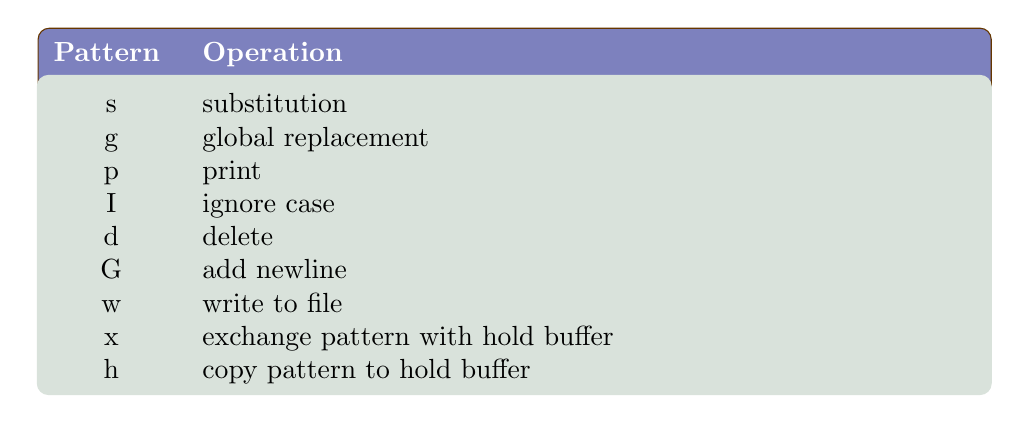
\begin{tikzpicture}
          \node (tbl) {
            \begin{tabularx}{\textwidth}{cl}
%              \arrayrulecolor{tigersgold}
              \textcolor{white}{\textbf{Pattern} }& \textcolor{white}{\textbf{Operation}} \\
              s\rule{0pt}{3.5ex} & substitution \\
              g & global replacement \\
              p & print \\
              I & ignore case \\
              d & delete \\
              G & add newline \\
              w & write to file\\
              x & exchange pattern with hold buffer\\
              h & copy pattern to hold buffer\\
              [1.0ex]
          \end{tabularx}};
          \begin{pgfonlayer}{background}
            \draw[rounded corners,top color=lupurple,bottom color=lupurple,
              draw=lubrown] ($(tbl.north west)+(0.14,0)$)
            rectangle ($(tbl.north east)-(0.13,0.9)$);
            \draw[rounded corners,top color=lulime,bottom color=lulime,draw=lulime]
            ($(tbl.north east)-(0.13,0.6)$)
            rectangle ($(tbl.south west)+(0.13,0.2)$);
          \end{pgfonlayer}
        \end{tikzpicture}
      \end{center} 
      \column{0.46\textwidth}
      \vspace{-0.6cm}
      \begin{center}
        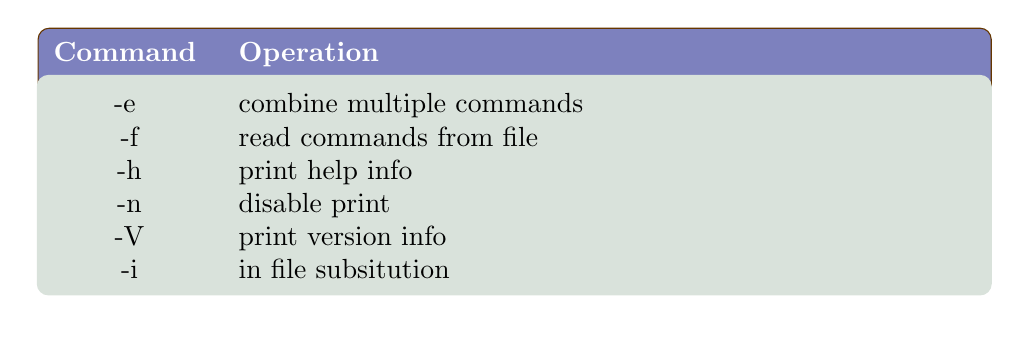
\begin{tikzpicture}
          \node (tbl) {
            \begin{tabularx}{\textwidth}{cl}
%              \arrayrulecolor{tigersgold}
              \textcolor{white}{\textbf{Command} }& \textcolor{white}{\textbf{Operation}} \\
              -e \rule{0pt}{3.5ex} & combine multiple commands \\
              -f & read commands from file \\
              -h & print help info \\
              -n & disable print \\
              -V & print version info \\
              -i & in file subsitution \\
              [1.0ex]
          \end{tabularx}};
          \begin{pgfonlayer}{background}
            \draw[rounded corners,top color=lupurple,bottom color=lupurple,
              draw=lubrown] ($(tbl.north west)+(0.14,0)$)
            rectangle ($(tbl.north east)-(0.13,0.9)$);
            \draw[rounded corners,top color=lulime,bottom color=lulime,draw=lulime]
            ($(tbl.north east)-(0.13,0.6)$)
            rectangle ($(tbl.south west)+(0.13,0.2)$);
          \end{pgfonlayer}
        \end{tikzpicture}
      \end{center} 
    \end{columns}
    \framebreak
    \item Add the \texttt{-e} to carry out multiple matches.
      \begin{lstlisting}[style=LINUX]
~/Tutorials/BASH/scripts/day1/examples> cat hello.sh | sed -e 's/bash/tcsh/g' -e 's/First/First tcsh/g'
#!/bin/tcsh

# My First tcsh Script

echo ``Hello World!''
      \end{lstlisting}
    \item Alternate forms
      \begin{lstlisting}[style=LINUX]
~/Tutorials/BASH/scripts/day1/examples> cat hello.sh | sed 's/bash/tcsh/g' | sed 's/First/First tcsh/g'
OR
~/Tutorials/BASH/scripts/day1/examples> sed 's/bash/tcsh/g; s/First/First tcsh/g' hello.sh 
#!/bin/tcsh

# My First tcsh Script

echo ``Hello World!''
      \end{lstlisting}
    \item The delimiter is slash (/). You can change it to whatever you want which is useful when you want to replace path names
      \begin{lstlisting}[style=LINUX]
~/Tutorials/BASH/scripts/day1/examples> sed 's:/bin/bash:/usr/bin/env tcsh:g' hello.sh 
#!/usr/bin/env tcsh

# My First Script

echo ``Hello World!''
      \end{lstlisting}
      \framebreak
    \item If you do not use an alternate delimiter, use backslash (\textbackslash) to escape the slash character in your pattern
      \begin{lstlisting}[style=LINUX]
~/Tutorials/BASH/scripts/day1/examples> sed 's/\/bin\/bash/\/usr\/bin\/env tcsh/g' hello.sh 
#!/usr/bin/env tcsh

# My First Script

echo ``Hello World!''
      \end{lstlisting}
    \item If you enter all your sed commands in a file, say sedscript, you can use the -f flag to sed to read the sed commands
      \begin{lstlisting}[style=LINUX]
~/Tutorials/BASH/scripts/day1/examples> cat sedscript
s/bash/tcsh/g
~/Tutorials/BASH/scripts/day1/examples> sed -f sedscript hello.sh 
#!/bin/tcsh

# My First Script

echo ``Hello World!''
      \end{lstlisting}
    \item sed can also delete blank files from a file
      \begin{lstlisting}[style=LINUX]
~/Tutorials/BASH/scripts/day1/examples> sed '/^$/d' hello.sh 
#!/bin/bash
# My First Script
echo ``Hello World!''
      \end{lstlisting}
    \item delete line n through m in a file
      \begin{lstlisting}[style=LINUX]
~/Tutorials/BASH/scripts/day1/examples> sed '2,4d' hello.sh 
#!/bin/bash
echo ``Hello World!''
      \end{lstlisting}
      \framebreak
      \item insert a blank line above every line which matches ``regex''
        \begin{lstlisting}[style=LINUX]
~/Tutorials/BASH/scripts/day1/examples> sed '/First/{x;p;x;}' hello.sh 
#!/bin/bash


# My First Script

echo ``Hello World!''
        \end{lstlisting}
      \item insert a blank line below every line which matches ``regex''
        \begin{lstlisting}[style=LINUX]
~/Tutorials/BASH/scripts/day1/examples> sed '/First/G' hello.sh 
#!/bin/bash

# My First Script


echo ``Hello World!''
        \end{lstlisting}
      \item insert a blank line above and below every line which matches ``regex''
        \begin{lstlisting}[style=LINUX]
~/Tutorials/BASH/scripts/day1/examples> sed '/First/{x;p;x;G;}' hello.sh 
#!/bin/bash


# My First Script


echo ``Hello World!''
        \end{lstlisting}
        \framebreak
    \item delete lines matching pattern regex
      \begin{lstlisting}[style=LINUX]
~/Tutorials/BASH/scripts/day1/examples> sed '/First/d' hello.sh 
#!/bin/bash


echo ``Hello World!''
      \end{lstlisting}
    \item print only lines which match regular expression (emulates grep)
      \begin{lstlisting}[style=LINUX]
~/Tutorials/BASH/scripts/day1/examples> sed -n '/echo/p' hello.sh
echo ``Hello World!''
      \end{lstlisting}
    \item print only lines which do NOT match regex (emulates grep -v)
      \begin{lstlisting}[style=LINUX]
~/Tutorials/BASH/scripts/day1/examples> sed -n '/echo/!p' hello.sh
#!/bin/bash

# My First Script

      \end{lstlisting}
    \item print current line number to standard output
      \begin{lstlisting}[style=LINUX]
~/Tutorials/BASH/scripts/day1/examples> sed -n '/echo/ =' quotes.sh 
5
6
7
8
9
10
11
12
13
      \end{lstlisting}
    \item If you want to make substitution in place, i.e. in the file, then use the -i command. If you append a suffix to -i, then the original file will be backed up as \textit{filename}suffix
      \begin{lstlisting}[style=LINUX,basicstyle=\fontsize{4}{5}\selectfont\ttfamily]
~/Tutorials/BASH/scripts/day1/examples> cat hello1.sh
#!/bin/bash

# My First Script

echo ``Hello World!''
~/Tutorials/BASH/scripts/day1/examples> sed -i.bak -e 's/bash/tcsh/g' -e 's/First/First tcsh/g' hello1.sh 
~/Tutorials/BASH/scripts/day1/examples> cat hello1.sh
#!/bin/tcsh

# My First tcsh Script

echo ``Hello World!''
~/Tutorials/BASH/scripts/day1/examples> cat hello1.sh.bak
#!/bin/bash

# My First Script

echo ``Hello World!''
      \end{lstlisting}
      \item double space a file
        \begin{lstlisting}[style=LINUX]
~/Tutorials/BASH/scripts/day1/examples> sed G hello.sh 
#!/bin/bash



# My First Script



echo ``Hello World!''

        \end{lstlisting}
        \framebreak
      \item double space a file which already has blank lines in it. Output file should contain no more than one blank line between lines of text.
        \begin{lstlisting}[style=LINUX]
~/Tutorials/BASH/scripts/day1/examples> sed '2,4d' hello.sh | sed '/^$/d;G'
#!/bin/bash

echo ``Hello World!''

        \end{lstlisting}
      \item triple space a file \texttt{sed 'G;G'}
      \item  undo double-spacing (assumes even-numbered lines are always blank)
        \begin{lstlisting}[style=LINUX]
~/Tutorials/BASH/scripts/day1/examples> sed 'n;d' hello.sh 
#!/bin/bash
# My First Script
echo ``Hello World!''
        \end{lstlisting}
    \item print the line immediately before or after a regexp, but not the line containing the regexp
      \begin{lstlisting}[style=LINUX]
apacheco@apacheco:~/Tutorials/BASH/scripts/day2/csplit> sed -n '/Normal/{g;1!p;};h' h2o-opt-freq.log 
 File lengths (MBytes):  RWF=      5 Int=      0 D2E=      0 Chk=      1 Scr=      1
 File lengths (MBytes):  RWF=      5 Int=      0 D2E=      0 Chk=      1 Scr=      1

apacheco@apacheco:~/Tutorials/BASH/scripts/day2/csplit> sed -n '/Normal/{n;p;}' h2o-opt-freq.log 
 (Enter /usr/local/packages/gaussian09/g09/l1.exe)
      \end{lstlisting}
      \framebreak
    \item print section of file between two regex:
      \begin{lstlisting}[style=LINUX]
~/Tutorials/BASH/scripts/day2/awk-sed> cat nh3-drc.out | sed -n '/START OF DRC CALCULATION/,/END OF ONE-ELECTRON INTEGRALS/p'
 START OF DRC CALCULATION
 ************************
 ---------------------------------------------------------------------------
   TIME     MODE     Q              P     KINETIC      POTENTIAL          TOTAL
    FS       BOHR*SQRT(AMU) BOHR*SQRT(AMU)/FS   E         ENERGY         ENERGY
    0.0000  L 1      1.007997  0.052824   0.00159      -56.52247      -56.52087
            L 2      0.000000  0.000000
            L 3     -0.000004  0.000000
            L 4      0.000000  0.000000
            L 5      0.000005  0.000001
            L 6     -0.138966 -0.014065
 ---------------------------------------------------------------------------
           CARTESIAN COORDINATES (BOHR)               VELOCITY (BOHR/FS)
 ---------------------------------------------------------------------------
  7.0     0.00000    0.00000    0.00000       0.00000    0.00000   -0.00616
  1.0    -0.92275    1.59824    0.00000       0.00000    0.00000    0.02851
  1.0    -0.92275   -1.59824    0.00000       0.00000    0.00000    0.02851
  1.0     1.84549    0.00000    0.00000       0.00000    0.00000    0.02851
 ---------------------------------------------------------------------------

                         ----------------------
                         GRADIENT OF THE ENERGY
                         ----------------------

 UNITS ARE HARTREE/BOHR    E'X               E'Y               E'Z 
    1 NITROGEN         0.000042455       0.000000188       0.000000000
    2 HYDROGEN         0.012826176      -0.022240529       0.000000000
    3 HYDROGEN         0.012826249       0.022240446       0.000000000
    4 HYDROGEN        -0.025694880      -0.000000105       0.000000000
 
 ...... END OF ONE-ELECTRON INTEGRALS ......
      \end{lstlisting}
      \framebreak
    \item print section of file from regex to end of file
      \begin{lstlisting}[style=LINUX]
~/Tutorials/BASH/scripts/day2/awk-sed> cat h2o-opt-freq.nwo | sed -n '/CITATION/,$p'
                                     CITATION
                                     --------

          Please use the following citation when publishing results
          obtained with NWChem:

          E. J. Bylaska, W. A. de Jong, N. Govind, K. Kowalski, T. P. Straatsma,
          M. Valiev, D. Wang, E. Apra, T. L. Windus, J. Hammond, P. Nichols,
          S. Hirata, M. T. Hackler, Y. Zhao, P.-D. Fan, R. J. Harrison,
          M. Dupuis, D. M. A. Smith, J. Nieplocha, V. Tipparaju, M. Krishnan,
          Q. Wu, T. Van Voorhis, A. A. Auer, M. Nooijen,
          E. Brown, G. Cisneros, G. I. Fann, H. Fruchtl, J. Garza, K. Hirao,
          R. Kendall, J. A. Nichols, K. Tsemekhman, K. Wolinski, J. Anchell,
          D. Bernholdt, P. Borowski, T. Clark, D. Clerc, H. Dachsel, M. Deegan,
          K. Dyall, D. Elwood, E. Glendening, M. Gutowski, A. Hess, J. Jaffe,
          B. Johnson, J. Ju, R. Kobayashi, R. Kutteh, Z. Lin, R. Littlefield,
          X. Long, B. Meng, T. Nakajima, S. Niu, L. Pollack, M. Rosing,
          G. Sandrone, M. Stave, H. Taylor, G. Thomas, J. van Lenthe, A. Wong,
          and Z. Zhang,
          ``NWChem, A Computational Chemistry Package for Parallel Computers, 
          Version 5.1'' (2007),
                      Pacific Northwest National Laboratory,
                      Richland, Washington 99352-0999, USA.



 Total times  cpu:        3.4s     wall:       18.5s

      \end{lstlisting}
      \framebreak
    \item sed one-liners: \url{http://sed.sourceforge.net/sed1line.txt}
    \item sed is a handy utility very useful for writing scripts for file manipulation.
  \end{itemize}
\end{frame}

\section{awk}
\begin{frame}[c,allowframebreaks,fragile]
%  \frametitle{awk}
  \begin{itemize}
%    \fontsize{7}{9}\selectfont{
    \item The Awk text-processing language is useful for such tasks as:
    \begin{enumerate}
      \item[$\bigstar$] Tallying information from text files and creating reports from the results.
      \item[$\bigstar$]Adding additional functions to text editors like "vi".
      \item[$\bigstar$] Translating files from one format to another.
      \item[$\bigstar$] Creating small databases.
      \item[$\bigstar$]Performing mathematical operations on files of numeric data.
    \end{enumerate}
    \item Awk has two faces: 
    \begin{enumerate}
      \item[$\bigstar$] it is a utility for performing simple text-processing tasks, and 
      \item[$\bigstar$] it is a programming language for performing complex text-processing tasks.
    \end{enumerate}
    \item awk comes in three variations
    \begin{enumerate}
        \item[awk]: Original AWK by A. Aho, B. W. Kernighnan and P. Weinberger
        \item[nawk]: New AWK, AT\&T's version of AWK
        \item[gawk]: GNU AWK, all linux distributions come with gawk. In some distros, awk is a symbolic link to gawk.
    \end{enumerate}
    \framebreak
    \item Simplest form of using awk
    \begin{enumerate}
      \item[$\vardiamond$]\textbf{awk} \textit{pattern} \{\texttt{action}\}
      \item[$\vardiamond$] Most common action: \texttt{print}
      \item[$\vardiamond$] Print file dosum.sh: \texttt{awk '\{print \$0\}' dosum.sh}
      \item[$\vardiamond$] Print line matching bash in all files in current directory:
      \item[] \texttt{awk '/bash/\{print \$0\}' *.sh }
    \end{enumerate}
    \item awk patterns may be one of the following
    \begin{description}
      {\scriptsize
        \item[BEGIN]: special pattern which is not tested against input.\\ Mostly used for preprocessing, setting constants, etc. before input is read.
        \item[END]: special pattern which is not tested against input.\\ Mostly used for postprocessing after input has been read.
        \item[/regular expression/]: the associated regular expression is matched to each input line that is read
        \item[relational expression]: used with the if, while relational operators
        \item[\&\& ]: logical AND operator used as pattern1 \&\& pattern2.\\ Execute action if pattern1 and pattern2 are true
        \item[$||$]: logical OR operator used as pattern1 || pattern2.\\ Execute action if either pattern1 or pattern2 is true
        \item[!]: logical NOT operator used as !pattern.\\ Execute action if pattern is not matched
        \item[?:]: Used as pattern1 ? pattern2 : pattern3.\\ If pattern1 is true use pattern2 for testing else use pattern3
        \item[pattern1, pattern2]: Range pattern, match all records starting with record that matches pattern1 continuing until a record has been reached that matches pattern2
      }
    \end{description}
    \framebreak
    \item Example: Print list of files that are csh script files
    \begin{lstlisting}[style=LINUX]
~/Tutorials/BASH/scripts/day1/examples> awk '/^#\!\/bin\/tcsh/{print FILENAME}' *
dooper.csh
factorial.csh
hello1.sh
name.csh
nestedloops.csh
quotes.csh
shift.csh
    \end{lstlisting}
    \item Example: Print contents of hello.sh that lie between two patterns
    \begin{lstlisting}[style=LINUX]
~/Tutorials/BASH/scripts/day1/examples> awk '/^#\!\/bin\/bash/,/echo/{print $0}' hello.sh
#!/bin/bash

# My First Script

echo ``Hello World!''
    \end{lstlisting}
    \framebreak
    \item awk reads the file being processed line by line. 
    \item The entire content of each line is split into columns with space or tab as the delimiter.
    \item By default the field separator is space or tab. To change the field separator use the -F command.
    \item To print the entire line, use \$0.
    \item The intrinsic variable NR contains the number of records (lines) read.
    \item The intrinsic variable NF contains the number of fields or columns in the current line.
    \begin{lstlisting}[style=LINUX]
~/Tutorials/BASH/scripts/day1/examples>awk '{print NR,'','',NF,'':'',$0}' hello.sh 
1 , 1 : #!/bin/bash
2 , 0 : 
3 , 4 : # My First Script
4 , 0 : 
5 , 3 : echo ``Hello World!''
~/Tutorials/BASH/scripts/day1/examples> uptime
 11:18am  up 14 days  0:40,  5 users,  load average: 0.15, 0.11, 0.17
apacheco@apacheco:~/Tutorials/BASH/scripts/day1/examples> uptime | awk '{print $1,$NF}'
11:19am 0.17
apacheco@apacheco:~/Tutorials/BASH/scripts/day1/examples> uptime | awk -F: '{print $1,$NF}'
 11  0.12, 0.10, 0.16
    \end{lstlisting}
    \framebreak
    \item \textit{print expression} is the most common action in the awk statement. If formatted output is required, use the \textit{printf format, expression} action.
    \item Format specifiers are similar to the C-programming language
    \begin{description}
      \fontsize{7}{9}\selectfont{
        \item[\%d,\%i]: decimal number
        \item[\%e,\%E]: floating point number of the form [-]d.dddddd.e[$\pm$]dd. The \%E format uses E instead of e.
        \item[\%f]: floating point number of the form [-]ddd.dddddd
        \item[\%g,\%G]: Use \%e or \%f conversion with nonsignificant zeros truncated. The \%G format uses \%E instead of \%e
        \item[\%s]: character string
      }
    \end{description}
    \item Format specifiers have additional parameter which may lie between the \% and the control letter
    \begin{description}
      \fontsize{7}{9}\selectfont{
      \item[0]: A leading 0 (zero) acts as a flag, that indicates output should be padded with zeroes instead of spaces.
      \item[width]: The field should be padded to this width. The field is normally padded  with  spaces.  If the 0 flag has been used, it is padded with zeroes.
      \item[.prec]: A number that specifies the precision to use when printing.
      }
    \end{description}
    \framebreak
    \item string constants supported by awk
    \begin{description}
      \fontsize{7}{9}\selectfont{
        \item[\textbackslash\textbackslash]: Literal backslash
        \item[{\textbackslash}n]: newline
        \item[{\textbackslash}r]: carriage-return
        \item[{\textbackslash}t]: horizontal tab
        \item[{\textbackslash}v]: vertical tab
      }
    \end{description}
    \begin{lstlisting}[style=LINUX]
~/Tutorials/BASH/scripts/day1/examples> echo hello 0.2485 5 | awk '{printf ``%s \t %f \n %d \v %0.5d\n'',$1,$2,$3,$3}'
hello    0.248500 
 5 
    00005
    \end{lstlisting}
    \item The print command puts an explicit newline character at the end while the printf command does not.
    \framebreak
    \item awk has in-built support for arithmetic operations
    \begin{columns}
      \column{0.5\textwidth}
    \begin{center}
      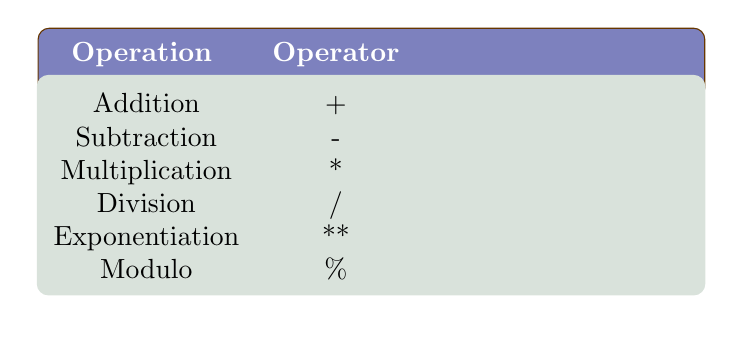
\begin{tikzpicture}
        \node (tbl) {
          \begin{tabularx}{0.7\textwidth}{cc}
            \arrayrulecolor{tigersgold}
            \textcolor{white}{\textbf{Operation} }& \textcolor{white}{\textbf{Operator}} \\
            Addition\rule{0pt}{3.5ex} & + \\
            Subtraction & - \\
            Multiplication & * \\
            Division & / \\
            Exponentiation & ** \\
            Modulo & \% \\
            [1.0ex]
        \end{tabularx}};
        \begin{pgfonlayer}{background}
          \draw[rounded corners,top color=lupurple,bottom color=lupurple,
            draw=lubrown] ($(tbl.north west)+(0.14,0)$)
          rectangle ($(tbl.north east)-(0.13,0.9)$);
          \draw[rounded corners,top color=lulime,bottom color=lulime,draw=lulime]
          ($(tbl.north east)-(0.13,0.6)$)
          rectangle ($(tbl.south west)+(0.13,0.2)$);
        \end{pgfonlayer}
      \end{tikzpicture}
    \end{center} 
      \column{0.5\textwidth}
      \vspace{-0.4cm}
    \begin{center}
      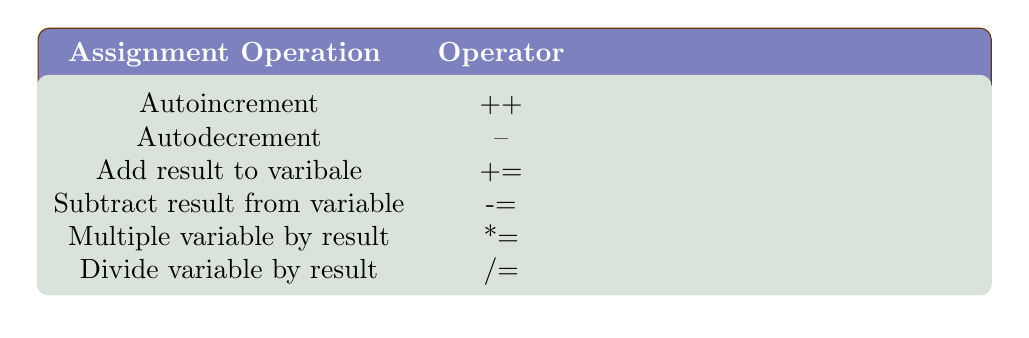
\begin{tikzpicture}
        \node (tbl) {
          \begin{tabularx}{\textwidth}{cc}
            \arrayrulecolor{tigersgold}
            \textcolor{white}{\textbf{Assignment Operation} }& \textcolor{white}{\textbf{Operator}} \\
            Autoincrement\rule{0pt}{3.5ex} & ++ \\
            Autodecrement & -- \\
            Add result to varibale & += \\
            Subtract result from variable & -= \\
            Multiple variable by result & *= \\
            Divide variable by result & /= \\
            [1.0ex]
        \end{tabularx}};
        \begin{pgfonlayer}{background}
          \draw[rounded corners,top color=lupurple,bottom color=lupurple,
            draw=lubrown] ($(tbl.north west)+(0.14,0)$)
          rectangle ($(tbl.north east)-(0.13,0.9)$);
          \draw[rounded corners,top color=lulime,bottom color=lulime,draw=lulime]
          ($(tbl.north east)-(0.13,0.6)$)
          rectangle ($(tbl.south west)+(0.13,0.2)$);
        \end{pgfonlayer}
      \end{tikzpicture}
    \end{center}
    \end{columns}
    \begin{lstlisting}[style=LINUX]
~/Tutorials/BASH/scripts/day1/examples> echo | awk '{print 10%3}'
1
~/Tutorials/BASH/scripts/day1/examples> echo | awk '{a=10;print a/=5}'
2
    \end{lstlisting}
    \item awk also supports trignometric functions such as sin(expr) and cos(expr) where expr is in radians and atan2(y/x) where y/x is in radians
    \begin{lstlisting}[style=LINUX]
~/Tutorials/BASH/scripts/day1/examples> echo | awk '{pi=atan2(1,1)*4;print pi,sin(pi),cos(pi)}'
3.14159 1.22465e-16 -1
    \end{lstlisting}
    \framebreak
    \item Other Arithmetic operations supported are
    \begin{description}
      \item[exp(expr)]: The exponential function
      \item[int(expr)]: Truncates to an integer
      \item[log(expr)]: The natural Logarithm function
      \item[sqrt(expr)]: The square root function
      \item[rand()]: Returns a random number $N$ between 0 and 1 such that $0\le N < 1$
      \item[srand(expr)]: Uses expr as a new seed for random number generator. If expr is not provided, time of day is used.
    \end{description}
    \item \textbf{awk} supports the if and while conditional and for loops
    \item if and while conditionals work similar to that in C-programming
    \begin{columns}
      \column{0.3\textwidth}
      \begin{exampleblock}{}
        \begin{lstlisting}[language=bash]
if ( condition ) {
  command1 ;
  command2
}
        \end{lstlisting}
      \end{exampleblock}
      \column{0.3\textwidth}
      \begin{exampleblock}{}
        \begin{lstlisting}[language=bash]
while ( condition ) {
  command1 ;
  command2
}
        \end{lstlisting}
      \end{exampleblock}
    \end{columns}
    \framebreak
    \item awk supports if ... else if .. else conditionals. 
    \begin{columns}
      \column{0.3\textwidth}
      \begin{exampleblock}{}
        \begin{lstlisting}[language=bash]
if (condition1) {
  command1 ;
  command2
} else if (condition2 ) {
  command3
}  else {
  command4
}
        \end{lstlisting}
      \end{exampleblock}
    \end{columns}
    \item Relational operators supported by if and while
    \begin{description}
%      \fontsize{6}{8}\selectfont{
        \item[==]: Is equal to
        \item[!=]: Is not equal to
        \item[$>$]: Is greater than
        \item[$>=$]: Is greater than or equal to
        \item[$<$]: Is less than
        \item[$<=$]: Is less than or equal to
        \item[$\sim$]: String Matches to
        \item[!$\sim$]: Doesn't Match
%      }
    \end{description}
    \begin{lstlisting}[style=LINUX]
~/Tutorials/BASH/scripts/day1/examples> awk '{if (NR > 0 ){print NR,'':'', $0}}' hello.sh 
1 : #!/bin/bash
2 : 
3 : # My First Script
4 : 
5 : echo ``Hello World!''
    \end{lstlisting}
    \item The for command can be used for processing the various columns of each line
    \begin{lstlisting}[style=LINUX]
~/Tutorials/BASH/scripts/day1/examples> echo $(seq 1 10) | awk 'BEGIN{a=6}{for (i=1;i<=NF;i++){a+=$i}}END{print a}'                                                                                 
61
    \end{lstlisting}
    \item Like all progamming languages, awk supports the use of variables. Like Shell, variable types do not have to be defined.
    \item awk variables can be user defined or could be one of the columns of the file being processed.
    \begin{lstlisting}[style=LINUX]
~/Tutorials/BASH/scripts/day1/examples> awk '{print $1}' hello.sh 
#!/bin/bash

#

echo

~/Tutorials/BASH/scripts/day1/examples> awk '{col=$1;print col,$2}' hello.sh 
#!/bin/bash 
 
# My
 
echo ``Hello
    \end{lstlisting}
    \item Unlike Shell, awk variables are referenced as is i.e. no \$ prepended to variable name.
    \item awk one-liners: \url{http://www.pement.org/awk/awk1line.txt}
%    }
  \end{itemize}
\end{frame}

\begin{frame}[c,allowframebreaks,fragile]%{awk programming language}
  \fontsize{7}{9}\selectfont{
  \begin{itemize}
    \item awk can also be used as a programming language.
    \item The first line in awk scripts is the shebang line (\#!) which indicates the location of the awk binary. Use \texttt{which awk} to find the exact location
    \item On my Linux desktop, the location is /usr/bin/awk.
    \item If unsure, just use /usr/bin/env awk
  \end{itemize}
  \begin{columns}
    \column{0.3\textwidth}
    \begin{exampleblock}{hello.awk}
      \lstinputlisting[language=bash]{./scripts/day2/examples/hello.awk}
    \end{exampleblock}
    \column{0.5\textwidth}
%    \begin{block}{}
      \begin{lstlisting}[style=LINUX]
~/Tutorials/BASH/scripts/day2/examples> ./hello.awk 
Hello World!
      \end{lstlisting}
%    \end{block}
  \end{columns}
  \begin{itemize}
    \item To support scripting, awk has several built-in variables, which can also be used in one line commands
    \begin{description}
      \fontsize{6}{8}\selectfont{
        \item[ARGC]: number of command line arguments
        \item[ARGV]: array of command line arguments
        \item[FILENAME]: name of current input file
        \item[FS]: field separator
        \item[OFS]: output field separator
        \item[ORS]: output record separator, default is newline
      }
    \end{description}
    \framebreak
    \item awk permits the use of arrays
    \item arrays are subscripted with an expression between square brackets ([$\cdots$])
      \begin{columns}
        \column{0.6\textwidth}
        \begin{exampleblock}{hello1.awk}
          \lstinputlisting[language=bash]{./scripts/day2/examples/hello1.awk}
        \end{exampleblock}
        \begin{lstlisting}[style=LINUX]
~/Tutorials/BASH/scripts/day2/examples> ./hello1.awk 
 Hello, World!
        \end{lstlisting}
      \end{columns}
    \item Use the delete command to delete an array element
    \item awk has in-built functions to aid writing of scripts
    \begin{description}
      \fontsize{6}{8}\selectfont{
        \item[length]: length() function calculates the length of a string.
        \item[toupper]: toupper() converts string to uppercase (GNU awk only)
        \item[tolower]: tolower() converts to lower case (GNU awk only)
        \item[split]: used to split a string. Takes three arguments: the string, an array and a separator
        \item[gsub]: add primitive sed like functionality. Usage gsub(/pattern/,"replacement pattern",string)
        \item[getline]: force reading of new line
      }
    \end{description}
    \item Similar to bash, GNU awk also supports user defined function
      \begin{columns}
        \column{0.6\textwidth}
        \begin{exampleblock}{}
          \begin{lstlisting}[language=bash]
#!/usr/bin/gawk -f
{
    if (NF != 4) {
        error(``Expected 4 fields'');
    } else {
        print;
    }
}
function error ( message ) {
    if (FILENAME != ``-'') {
        printf(``%s: ``, FILENAME) > ``/dev/tty'';
    }
    printf(``line # %d, %s, line: %s\n'', NR, message, $0) >> ``/dev/tty'';
}
          \end{lstlisting}
        \end{exampleblock}
      \end{columns}
  \end{itemize}
  }
\end{frame}

\begin{frame}[c,allowframebreaks,fragile]%{Example Scripts}
  \begin{exampleblock}{getcpmdvels.sh}
    \lstinputlisting[language=bash,firstline=1,lastline=64,basicstyle=\fontsize{3}{3}\selectfont\ttfamily]{./scripts/day2/awk-sed/getcpmdvels.sh}
  \end{exampleblock}
  \begin{exampleblock}{getengcons.sh}
    \lstinputlisting[language=bash,firstline=1,lastline=64,basicstyle=\fontsize{3}{3}\selectfont\ttfamily]{./scripts/day2/awk-sed/getengcons.sh}
  \end{exampleblock}
%  \begin{exampleblock}{getcoordvels.sh}
    \lstinputlisting[language=bash,firstline=1,lastline=86,basicstyle=\fontsize{3}{3}\selectfont\ttfamily]{./scripts/day2/awk-sed/getcoordvels.sh}
%  \end{exampleblock}
    \framebreak
  \begin{exampleblock}{getmwvels.awk}
    \lstinputlisting[language=awk,firstline=1,lastline=64,basicstyle=\fontsize{3}{3}\selectfont\ttfamily]{./scripts/day2/awk-sed/getmwvels.awk}
  \end{exampleblock}
  \begin{exampleblock}{gettrajxyz.awk}
    \lstinputlisting[language=awk,firstline=1,lastline=64,basicstyle=\fontsize{3}{3}\selectfont\ttfamily]{./scripts/day2/awk-sed/gettrajxyz.awk}
  \end{exampleblock}
\end{frame}

\section{Wrap Up}
\begin{frame}
  \frametitle{References \& Further Reading}
  \begin{itemize}
    \fontsize{7}{9}\selectfont{
    \item BASH Programming \url{http://tldp.org/HOWTO/Bash-Prog-Intro-HOWTO.html}
    \item Advanced Bash-Scripting Guide \url{http://tldp.org/LDP/abs/html/}
    \item Regular Expressions \url{http://www.grymoire.com/Unix/Regular.html}
    \item AWK Programming \url{http://www.grymoire.com/Unix/Awk.html}
    \item awk one-liners: \url{http://www.pement.org/awk/awk1line.txt}
    \item sed \url{http://www.grymoire.com/Unix/Sed.html}
    \item sed one-liners: \url{http://sed.sourceforge.net/sed1line.txt}
    \item CSH Programming \url{http://www.grymoire.com/Unix/Csh.html}
    \item csh Programming Considered Harmful \url{http://www.faqs.org/faqs/unix-faq/shell/csh-whynot/}
    \item Wiki Books \url{http://en.wikibooks.org/wiki/Subject:Computing}
    }
  \end{itemize}
\end{frame}

\end{document}

